



\iffalse

Finally, at the end of the day, we are interested in learning about the underlying transverse quark distribution inside of
nucleons. A fellow graduate student in Richard Milner’s group, Yimin Wang, recently defended his thesis which included the
use of non-parameteric methods to extract the radius of the proton from various collider experiments. Similar methodology
can be employed to the finalized results of this and other DVπ0P experiments to estimate the parameters of the distribution
of valence quarks. Also, rosenbluth separation methods will be employed to extract parameters between this experiment and
lower energy runnings done in the past decade to further results in this space. Work is ongoing on this, and the other two areas
mentioned above, to extract meaningful data from this process, and better understand quark mechanics inside of nucleons.

absoulute normalization needs to go somwehere

\fi

\iffalse
Work is ongoing collaboration-wide to verify the absolute scale of the cross section measurement in reference to other reactions. Here we compare to CLAS6 result instead for cross check. 
\fi

\section{Cross Section Results}\label{sec:Ch5_raw_results}
%Include here just the bin by bin and unfolded cross sections and fits to dtaapoints no clas6 data, no GK model
    \subsection{Summary of Uncertainties}
        Major sources of systematic uncertainties are presented in table \ref{table:systematic_uncertainties} with their typical scale and if they are calculated for each bin or overall. The total systematic uncertainty is reported as the quadrature sum of the individual uncertainties, and is in-line with similar recent results \parencite{Lee2022MeasurementDetector}.

    \begin{table}[H]
        \centering
        \begin{tabular}{rcc}
        \hline
        Systematic Uncertainty & Median Percent Value & Bin or Overall \\ 
        \hline
            Fiducial Cuts / PID              & 12.3 \%    & Bin-by-bin   \\ 
            Reconstruction Efficiency       & 8.0 \%       & Bin-by-bin   \\ 
            Simulation Resolution Matching    & 8.6 \%       & Bin-by-bin   \\ 
            Exclusivity Cuts            & 12.4 \%      & Bin-by-bin   \\ 
            Acceptance Correction       & 9.8 \%       & Bin-by-bin   \\ 
            Radiative Correction        & 5.1 \%       & Bin-by-bin   \\ 
            Finite Bin Width            & 3.2 \%       & Bin-by-bin   \\
            Unfolding Methods            & 13.4 \%       & Bin-by-bin   \\ 
            Accumulated Beam Charge     & $<$1 \%        & Overall      \\ 
            Physical Target Properties  & $<$1\%    & Overall      \\
            Absolute Normalization      & 13\%       & Overall      \\ 
            \hline
            \textbf{Total (quadrature)}          & 30\%     & Bin-by-bin      \\ 
                \hline
        \end{tabular}
        \caption[Major Systematic Uncertainties]{Systematic uncertainties, their median percent values, and their calculation type.}
        \label{table:systematic_uncertainties}
    \end{table}

\iffalse

\begin{table}[h]
    \centering
    \begin{tabular}{rcc}
         %& Heading 1 & Heading 2 \\\hline
        Quantity & Symbol & CLAS12 Value \\\hline
       Avogadro's Number &  N$_A$  & 6.02214 x $10^{23}$ \\
        Electron Charge &e  &  1.602 x 10$^{-19}$ Coulombs \\
        Target Length &l &  5.00 cm \\
        Target Density &$\rho$  &  0.07 $g/cm^3$ (LH2) \\
        Charge on Faraday Cup & $Q_{FCUP}$ &  In data\\
    \end{tabular}
\caption[Terms of Luminosity Equation]{Values of terms in luminosity determination.}
\end{table}\label{lumitable}
\fi

    \iffalse

    from sangbaek

        
        Eqn. 5.24 assumed that the statistical uncertainty from generated events is negligible.
        The statistical uncertainty for the background estimation was assigned to the
        contamination ratio $c$, as discussed in Section 5.4.
        The major sources of systematic uncertainties include the inefficiency drop as a
        function of increasing beam current, over- or underestimation of the smearing parameter,
        over- or underestimation of the $\pi^0$ background, and the radiative corrections.
        Alternative exclusivity cuts at $2\sigma$ (Table 5.9) and $4\sigma$ ranges (Table 5.10) were applied
        to investigate the systematic uncertainties. Additionally, the individual particle
        selection cuts can have different impacts in the experimental data and the simulation
        data. The most unstable cuts are the CD proton polar angle ceiling cut ($64.23^\circ$), and
        the electron sampling fraction cut. The CD proton ceiling was adjusted to $59.23^\circ$
        and the electron sampling fraction cut of $3.5\sigma$ range was refined to $3\sigma$ to test the
        systematic effects. The resolution matching quality can affect the systematics, so the
        smearing parameter adjusted by 90\% and 110\% was applied to the total cross section
        contributions. The systematic uncertainty due to the $\pi^0$ background can be determined
        by estimating $\frac{N(e'p'2\gamma)DV\pi^0P_{exp}}{N(e'p'2\gamma)DV\pi^0P_{sim}}$
        in different ways ---bin-by-bin, or averaged in the
        entire kinematics region. The beam current contribution was estimated by simulating
        the DVCS and the DV$\pi^0$P events at different background merging currents.
        The systematic uncertainties in the unpolarized cross sections are summarized in
        Table 5.11.

    \fi


    \subsection{Reduced Cross Sections Across \texorpdfstring{$\phi$}{Phi}}
    
        Reduced cross section results are shown for bins across $x_B$, $Q^2$, and t in Figs. \ref{fig:combined_t0.2} - \ref{fig:combined_t1.5} with $x_B$ bins increasing from left to right and $Q^2$ bins increasing from bottom to top on a given page, and t bins increasing as page number increases. There were 1841 total 4-fold differential bins that passed all selection criteria. The features of each subfigure are as described in \figref{fig:binbybinIBU}. The fit on each subfigure is to the unfolded cross section result, rather than the bin-by-bin result. Note that distributions are only shown here that have enough coverage in $\phi$ to allow for a reasonable structure function curve fit. %The complete cross section results are tabulated in Appendix \ref{app:Across_sections}.
        
        \begin{figure}[ht]
            \centering
            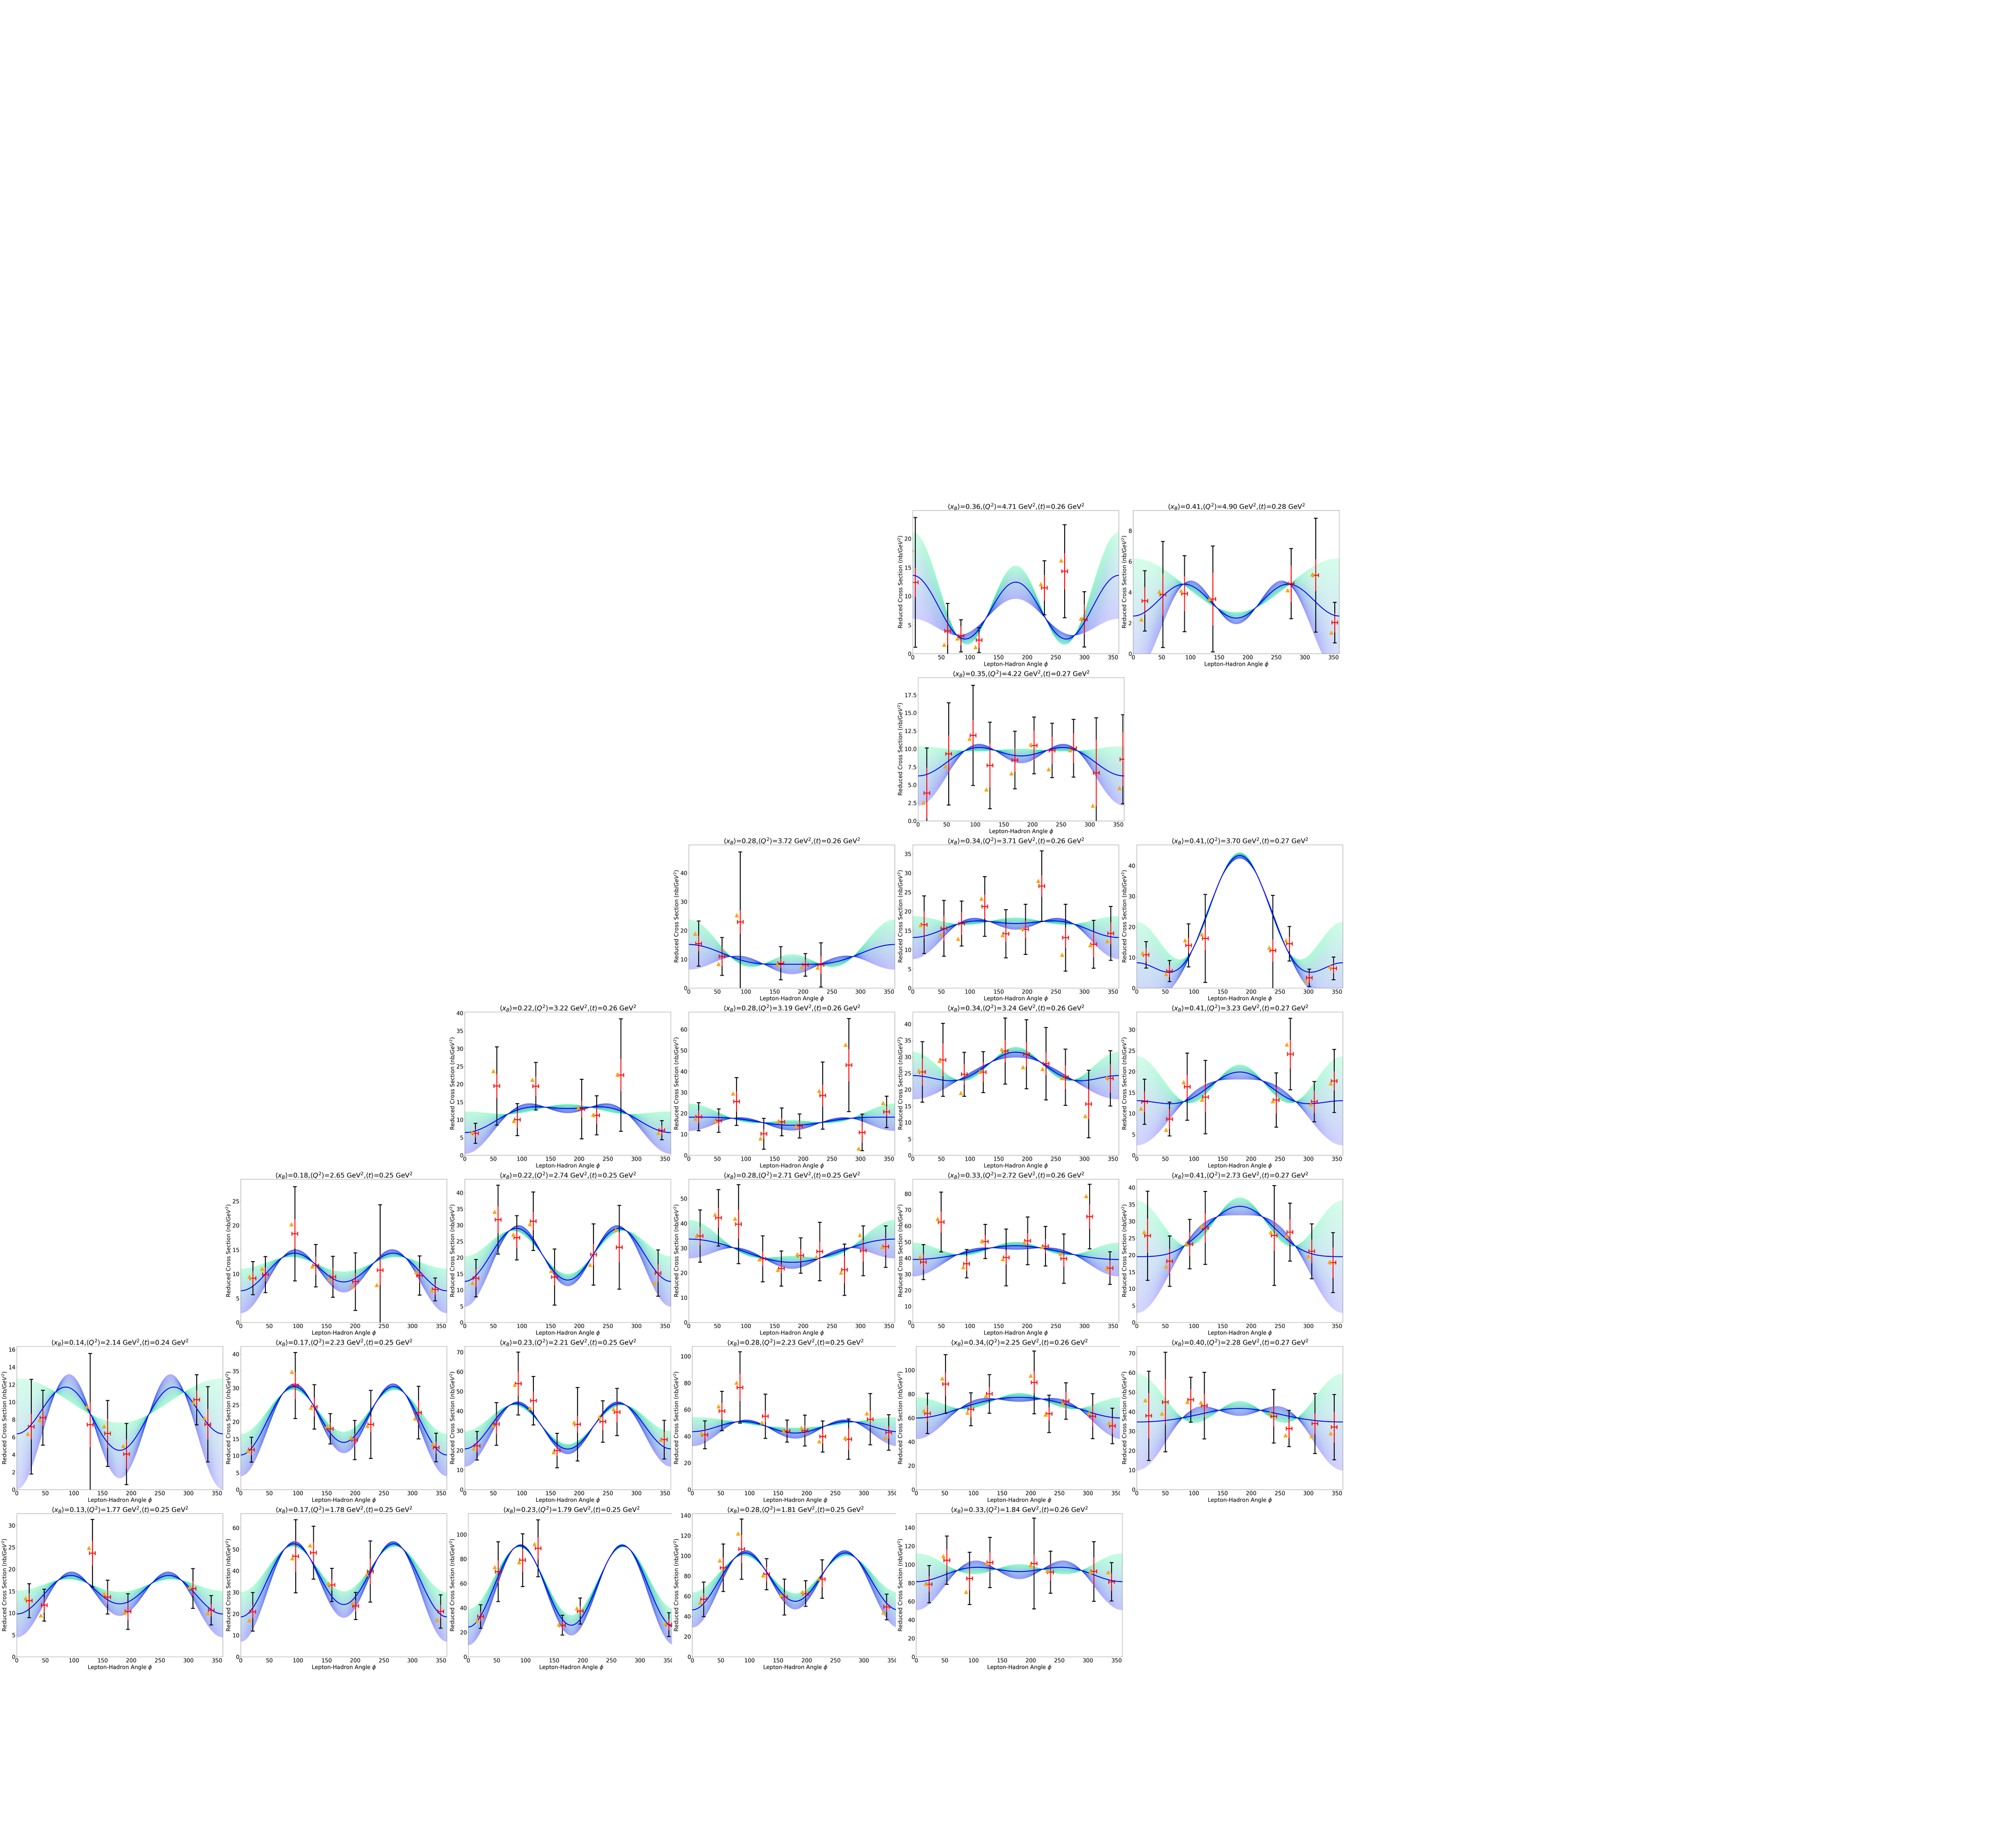
\includegraphics[trim={14.6cm 4cm 27.2cm 4cm},clip,width=0.8\textwidth]{Chapters/Ch5-Further/c12xsec/combined_t0.2.png}
            \caption[Reduced Cross Section for 0.2 $GeV^2 < t <$ 0.3 $ GeV^2$]{Reduced Cross Section for 0.2 $ GeV^2 < t <$ 0.3 $GeV^2$ in bins of $x_B$ (increasing left to right) and $Q^2$ (increasing vertically upwards). }
            \label{fig:combined_t0.2}
        \end{figure}
    
        \begin{figure}[ht]
            \centering
            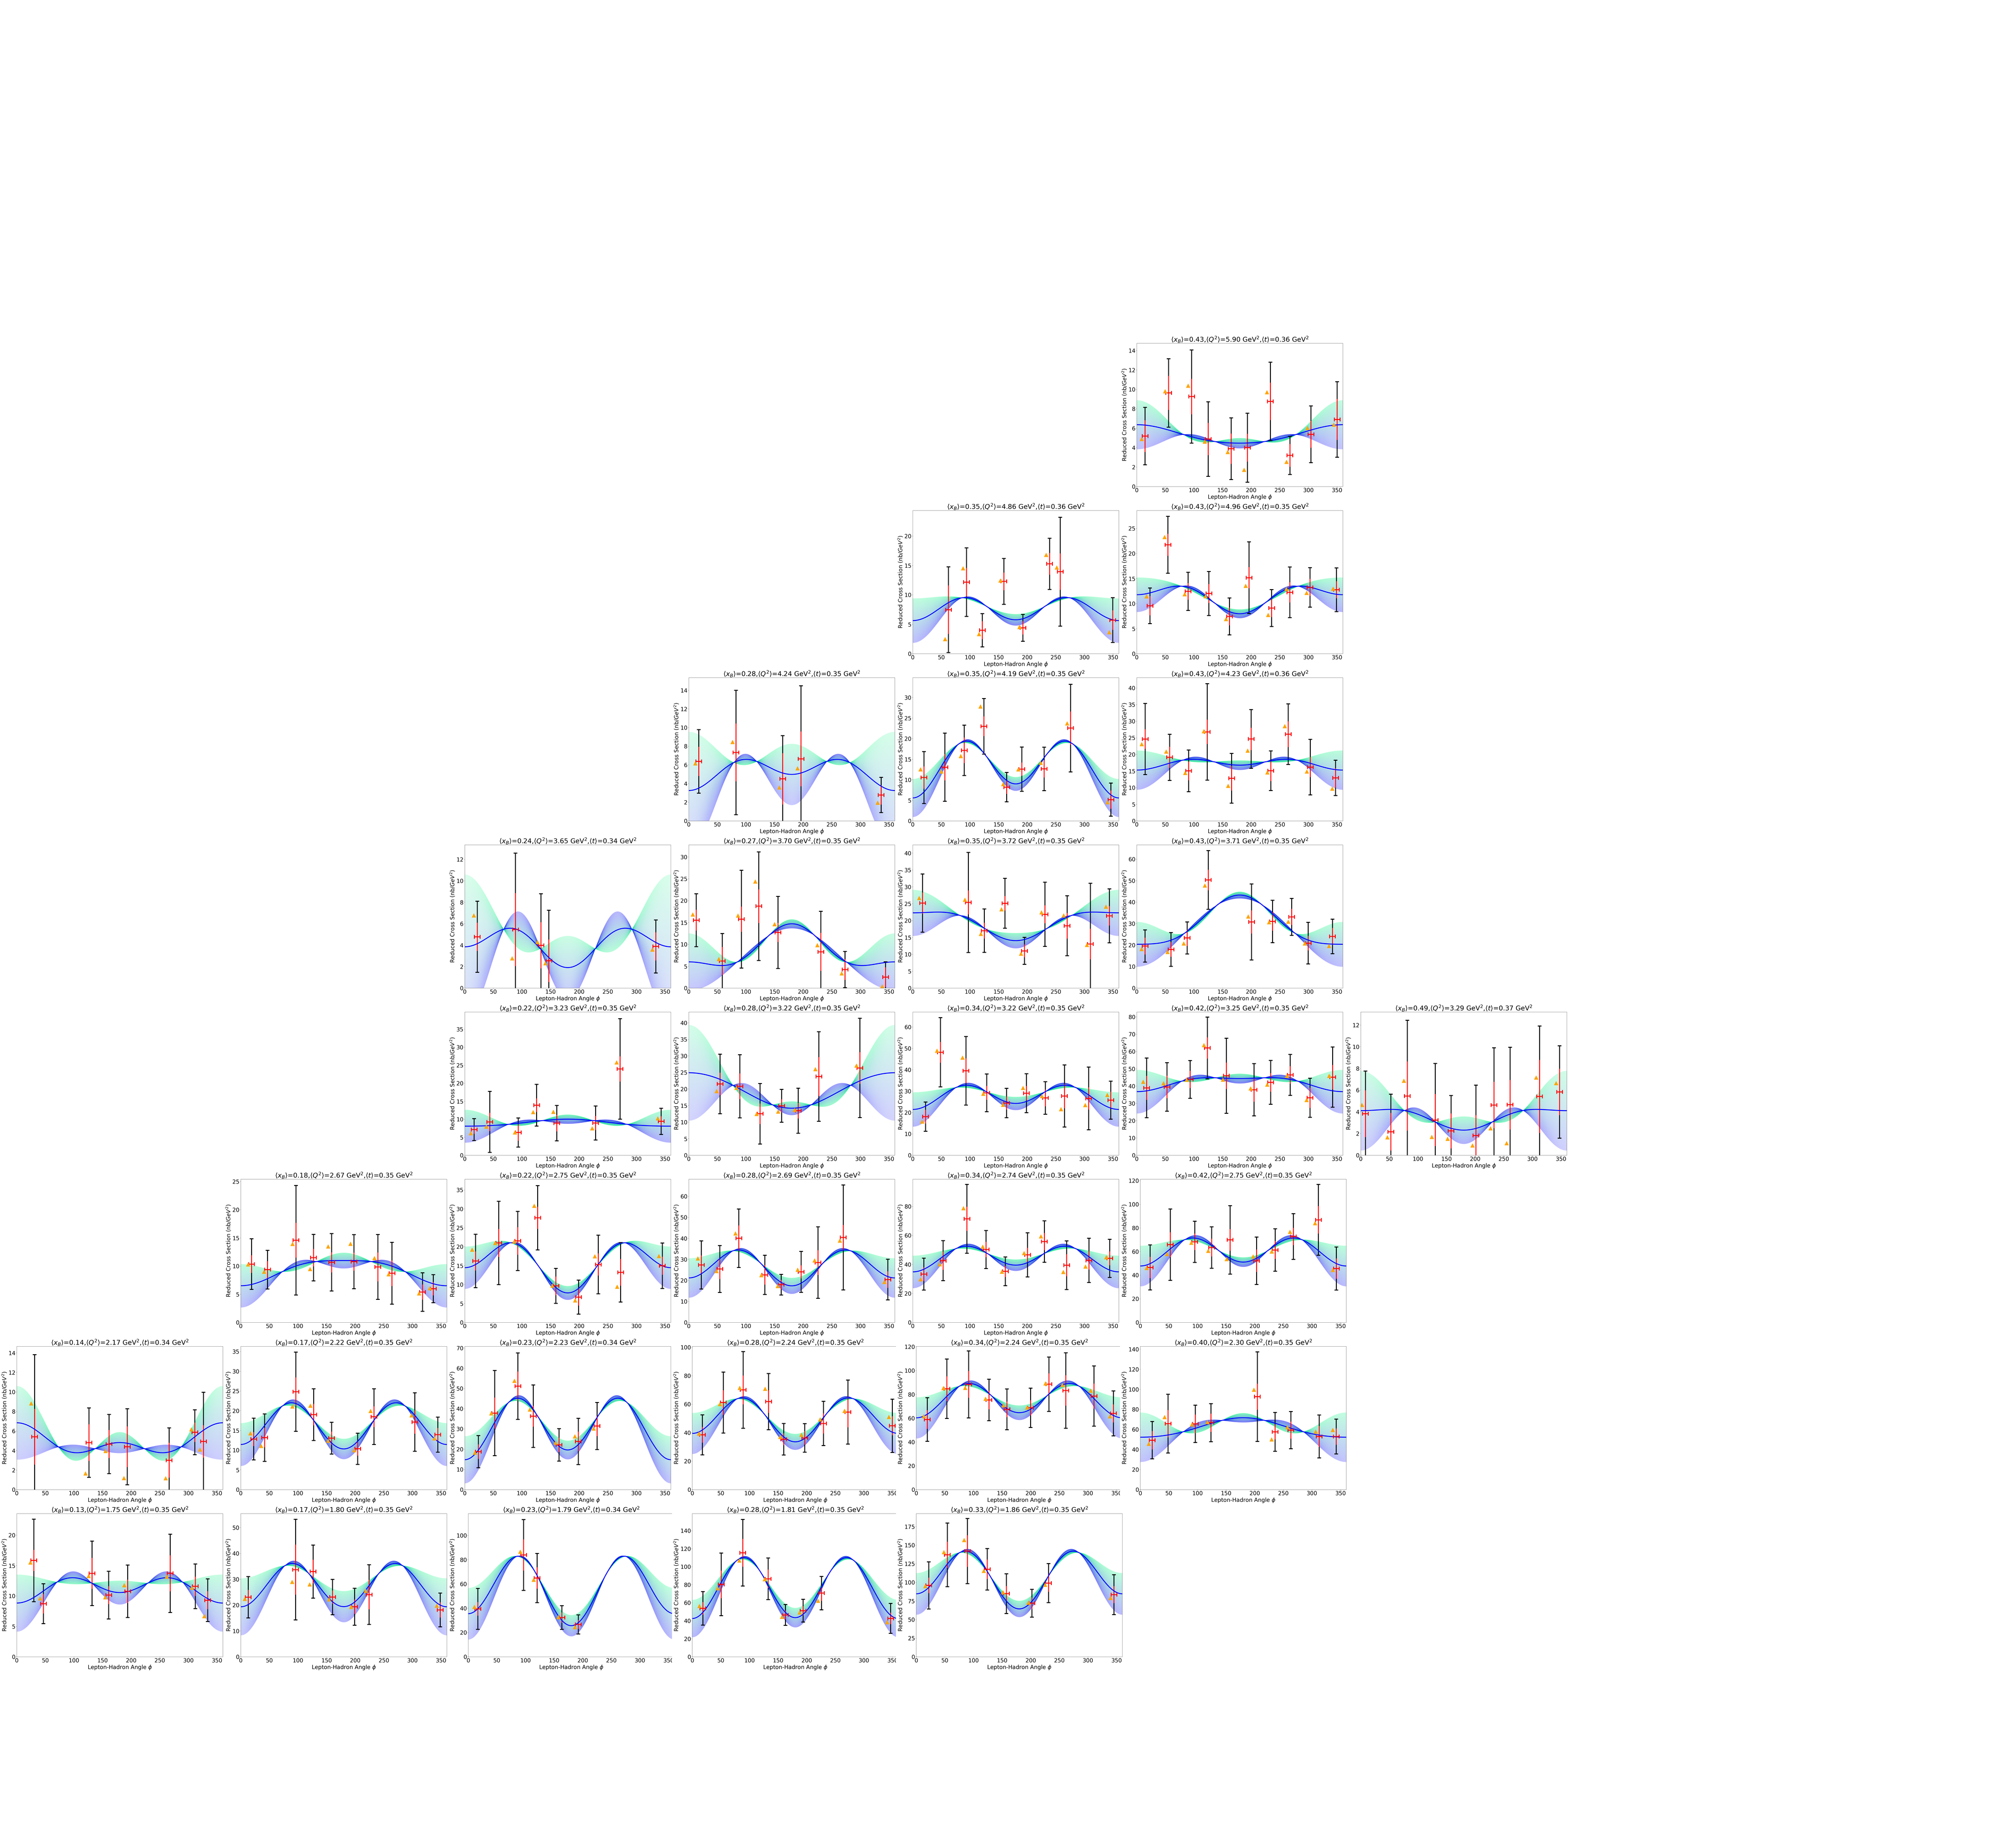
\includegraphics[trim={14.6cm 4cm 27.2cm 4cm},clip,width=0.8\textwidth]{Chapters/Ch5-Further/c12xsec/combined_t0.3.png}
            \caption[Reduced Cross Section for 0.3 $GeV^2 < t <$ 0.4 $ GeV^2$]{Reduced Cross Section for 0.3 $ GeV^2 < t <$ 0.3 $GeV^2$ in bins of $x_B$ (increasing left to right) and $Q^2$ (increasing vertically upwards). }
            \label{fig:combined_t0.3}
        \end{figure}
    
        \begin{figure}[ht]
            \centering
            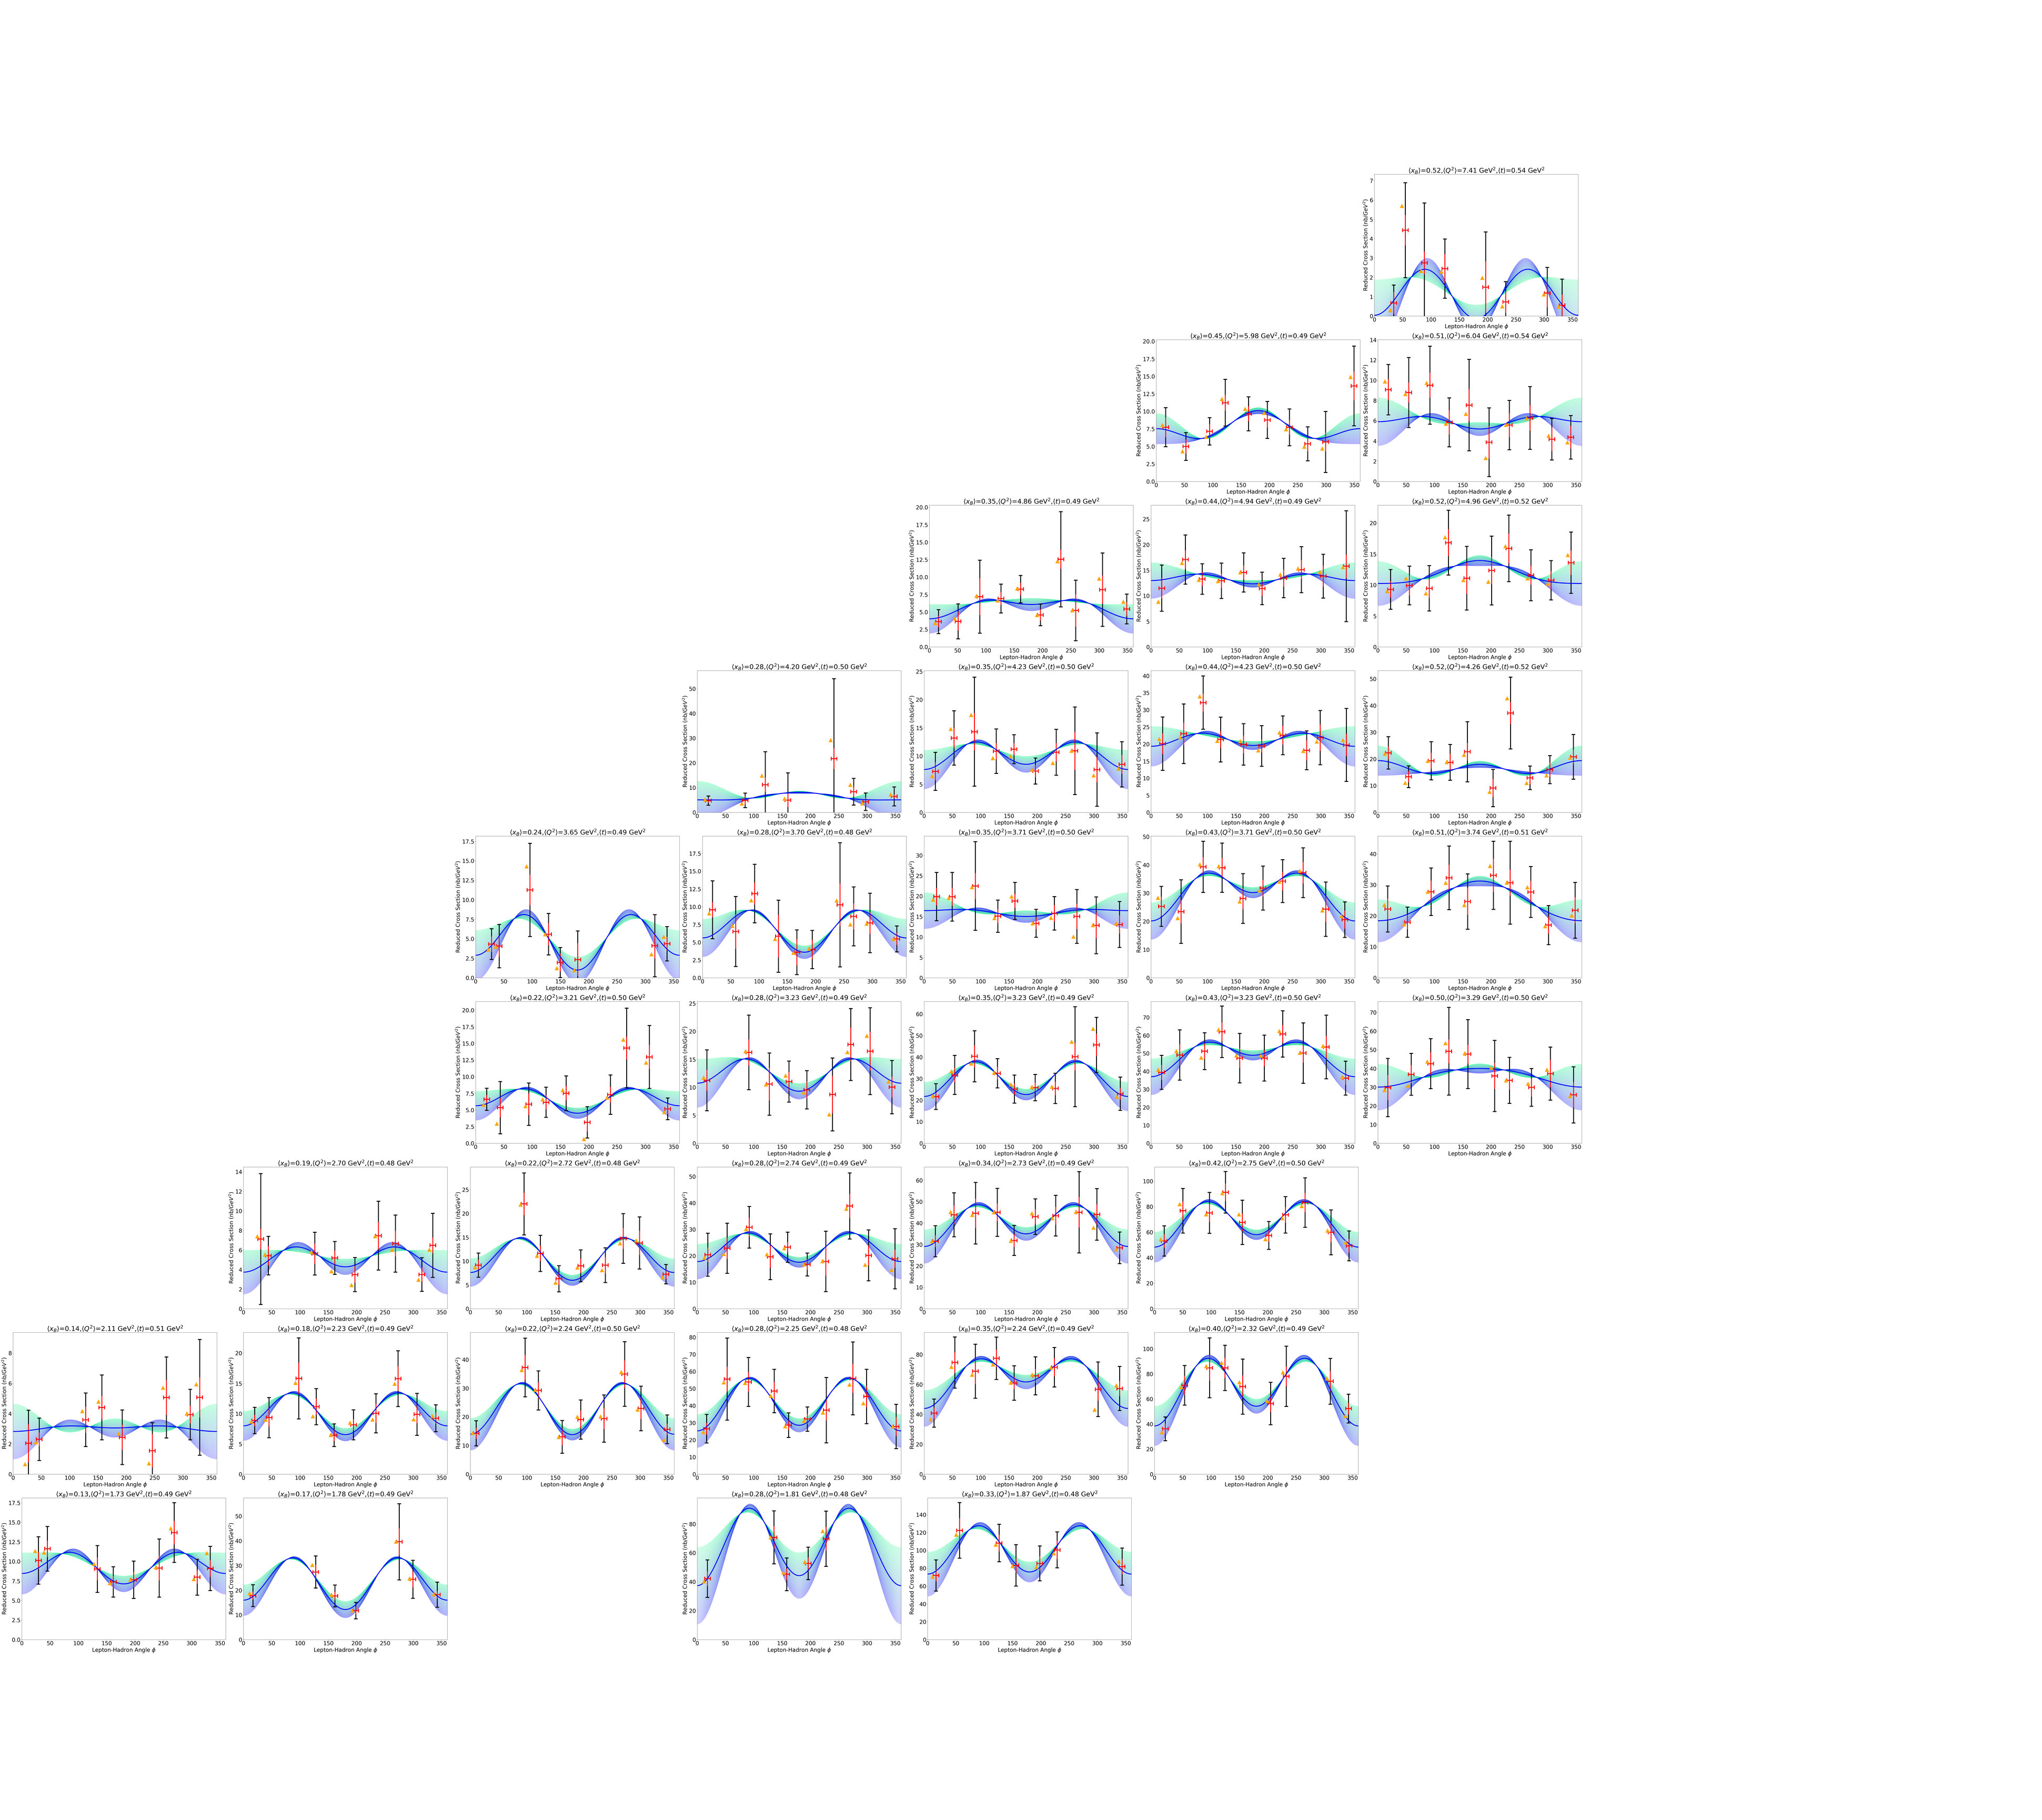
\includegraphics[trim={14.6cm 4cm 27.2cm 4cm},clip,width=0.8\textwidth]{Chapters/Ch5-Further/c12xsec/combined_t0.4.png}
            \caption[Reduced Cross Section for 0.4 $GeV^2 < t <$ 0.6 $ GeV^2$]{Reduced Cross Section for 0.4 $ GeV^2 < t <$ 0.6 $GeV^2$ in bins of $x_B$ (increasing left to right) and $Q^2$ (increasing vertically upwards). }
            \label{fig:combined_t0.4}
        \end{figure}
        
        \begin{figure}[ht]
            \centering
            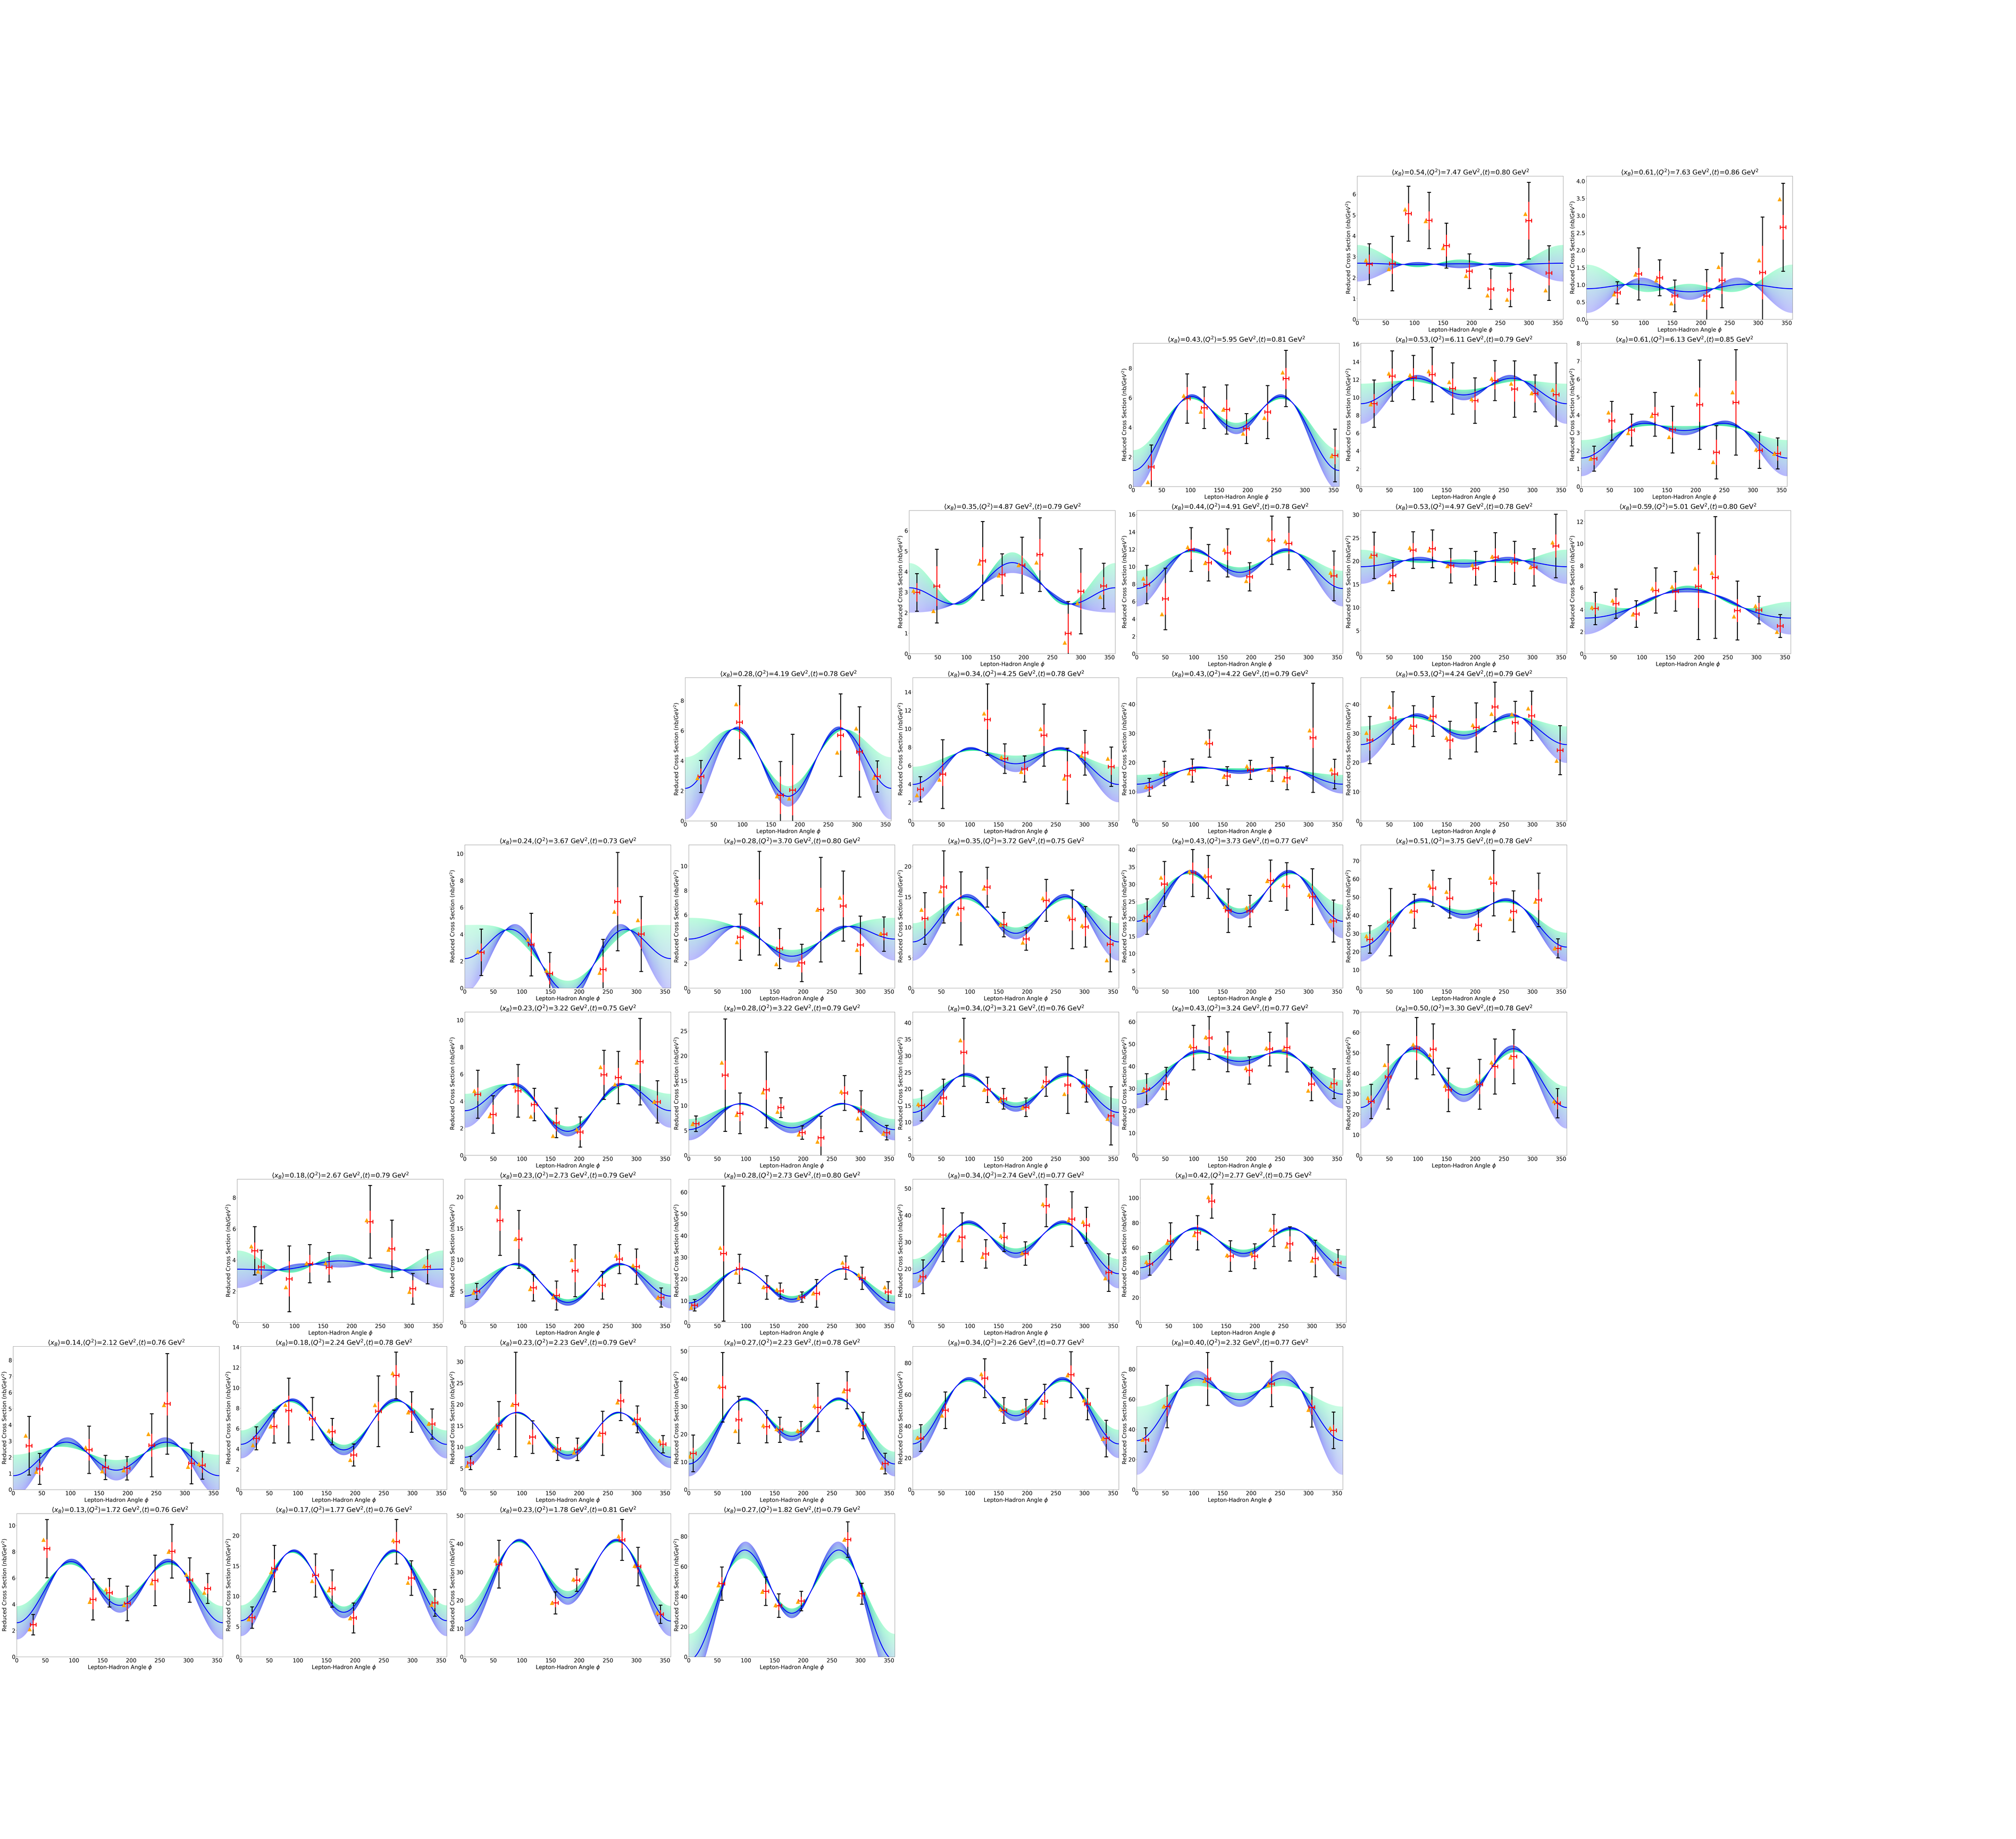
\includegraphics[trim={14.6cm 4cm 15.2cm 4cm},clip,width=0.8\textwidth]{Chapters/Ch5-Further/c12xsec/combined_t0.6.png}
            \caption[Reduced Cross Section for 0.6 $GeV^2 < t <$ 1.0 $ GeV^2$]{Reduced Cross Section for 0.6 $ GeV^2 < t <$ 1.0 $GeV^2$ in bins of $x_B$ (increasing left to right) and $Q^2$ (increasing vertically upwards). }
            \label{fig:combined_t0.6}
        \end{figure}
        
        \begin{figure}[ht]
            \centering
            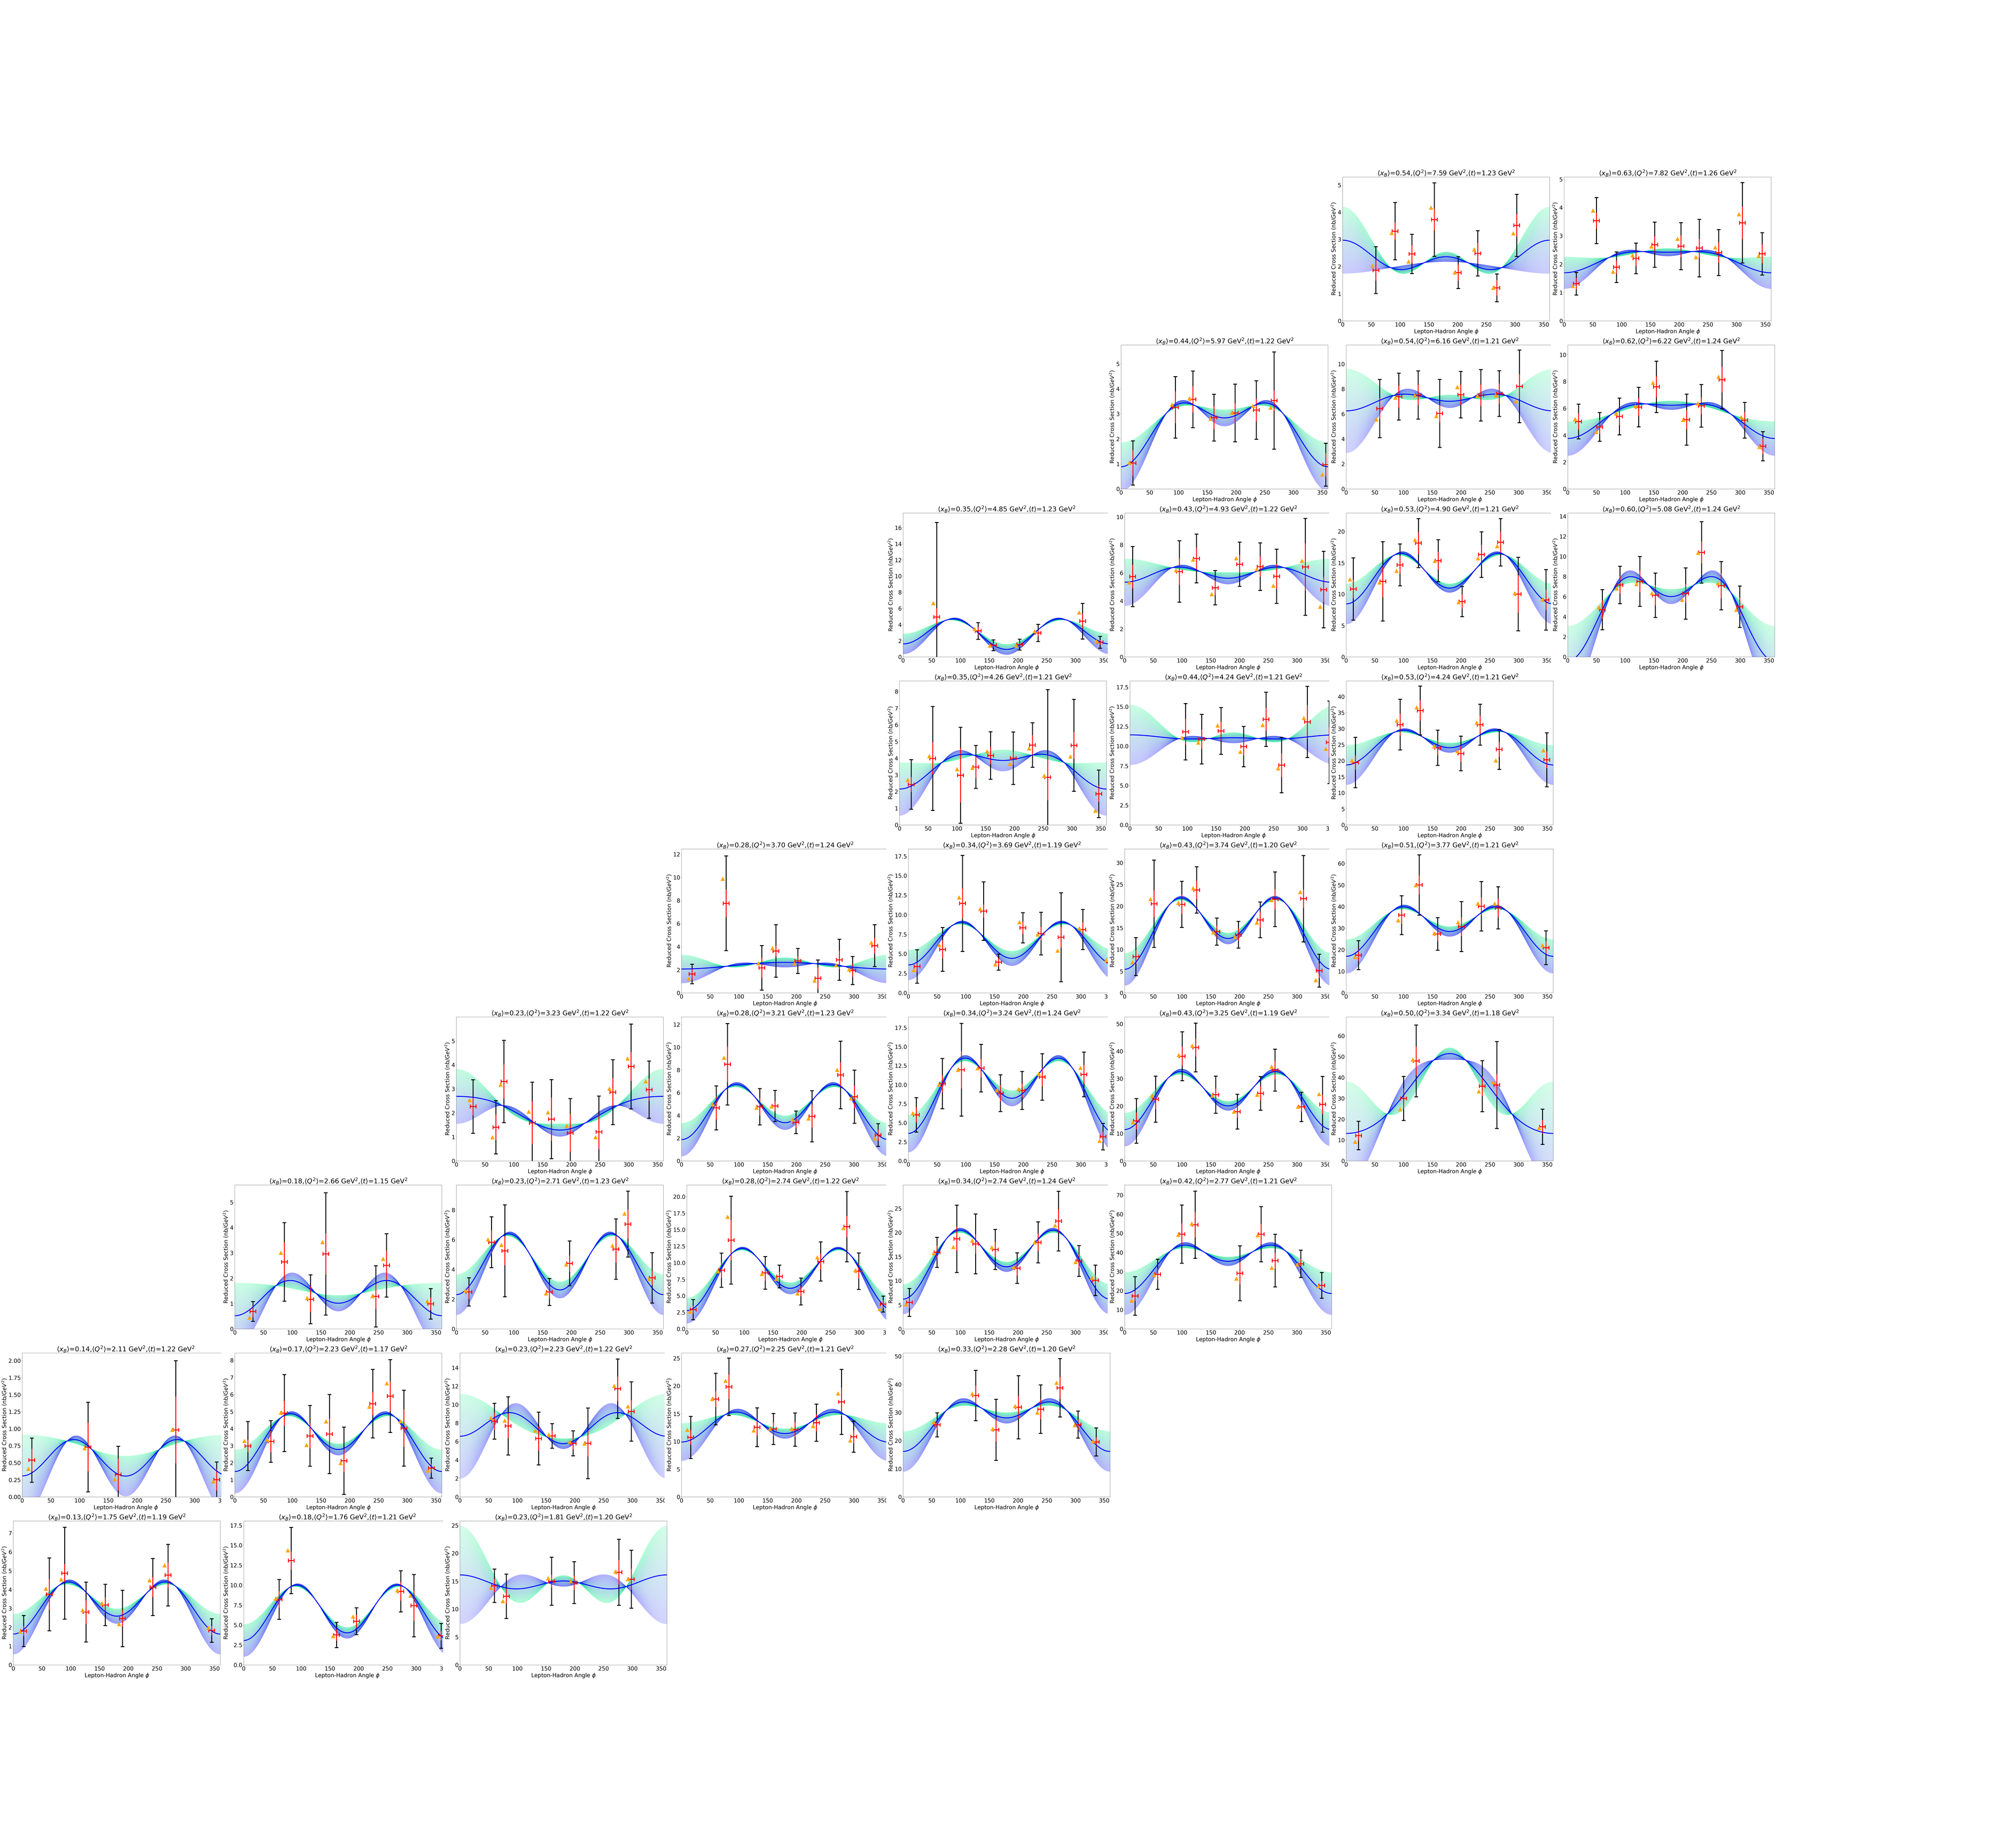
\includegraphics[trim={14.6cm 4cm 15.2cm 4cm},clip,width=0.8\textwidth]{Chapters/Ch5-Further/c12xsec/combined_t1.0.png}
            \caption[Reduced Cross Section for 1.0 $GeV^2 < t <$ 1.5 $ GeV^2$]{Reduced Cross Section for 1.0 $ GeV^2 < t <$ 1.5 $GeV^2$ in bins of $x_B$ (increasing left to right) and $Q^2$ (increasing vertically upwards). }
            \label{fig:combined_t1.0}
        \end{figure}
        
        \begin{figure}[ht]
            \centering
            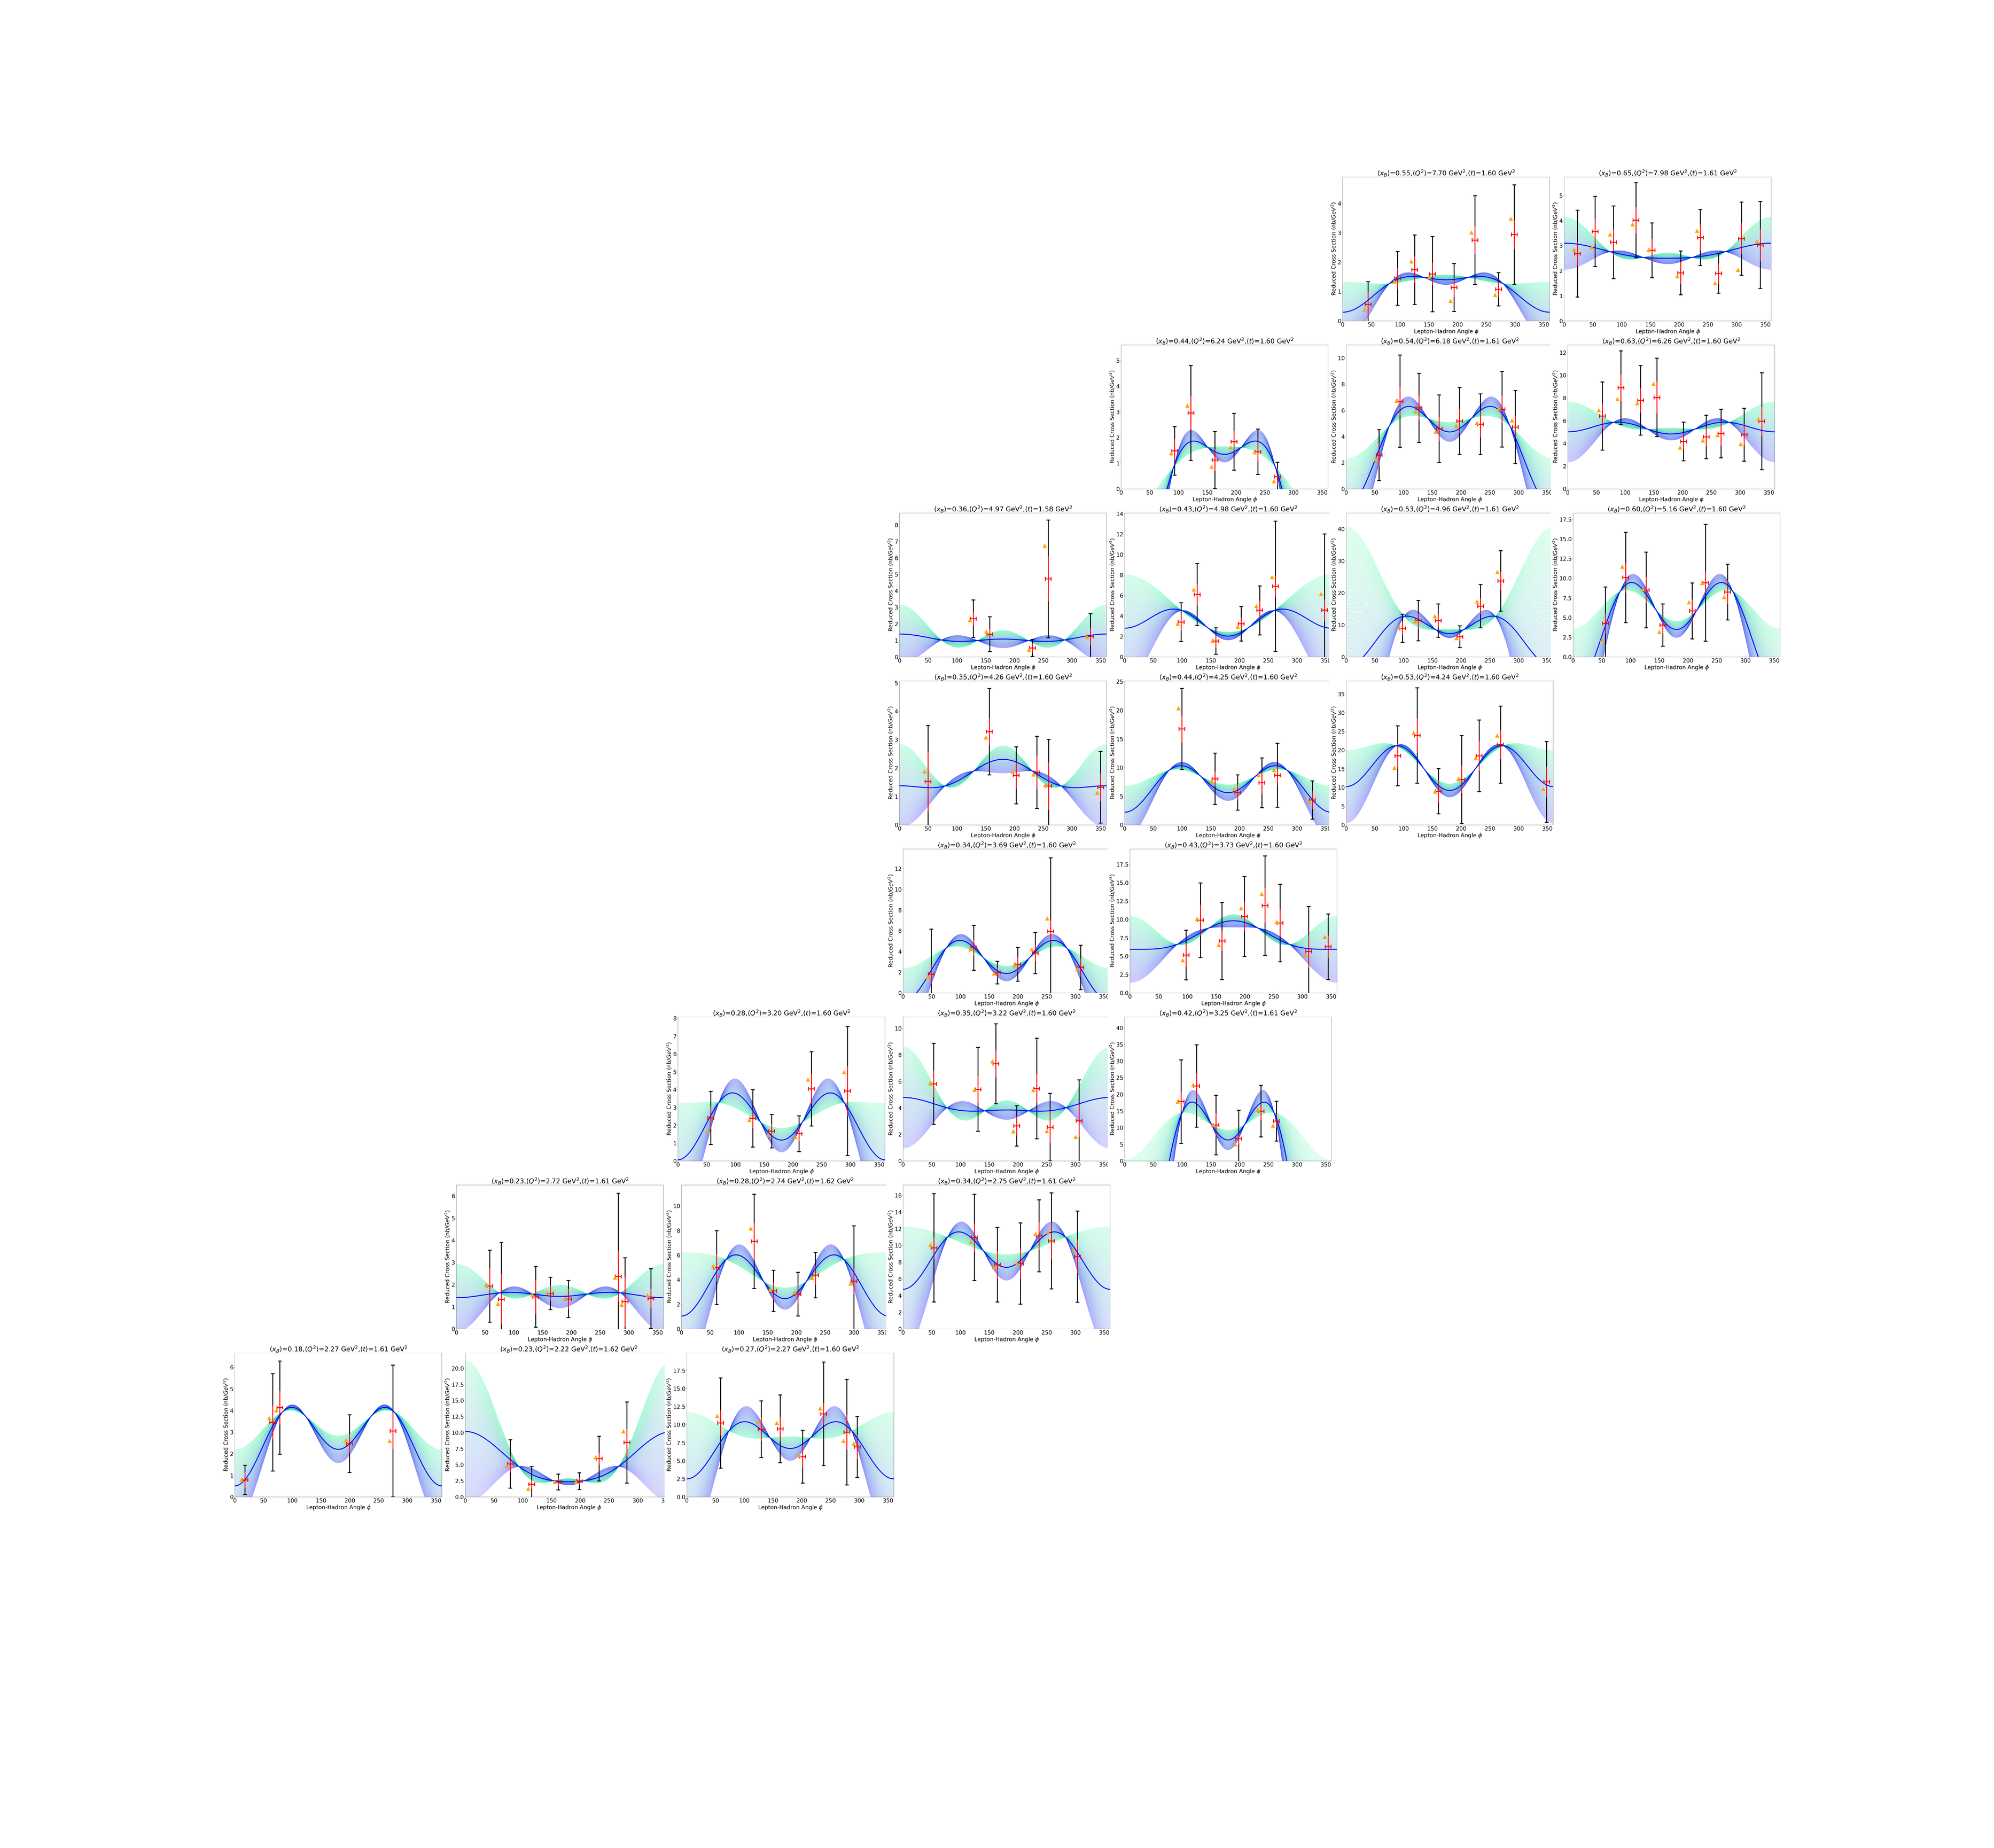
\includegraphics[trim={14.6cm 4cm 15.2cm 4cm},clip,width=0.8\textwidth]{Chapters/Ch5-Further/c12xsec/combined_t1.5.png}
            \caption[Reduced Cross Section for 1.5 $GeV^2 < t <$ 2.0 $ GeV^2$]{Reduced Cross Section for 1.5 $ GeV^2 < t <$ 2.0 $GeV^2$ in bins of $x_B$ (increasing left to right) and $Q^2$ (increasing vertically upwards). }
            \label{fig:combined_t1.5}
        \end{figure}

    \clearpage

\section{Structure Function Extraction}

    As discussed, the \xsec for this process can be expressed in terms of structure functions as \ref{eq:DVPiPCrossSection_theory}
    
        \begin{equation*}
             \recallLabel{eq:DVPiPCrossSection_theory}
        \end{equation*}

    The  A+B$\cos{2\phi}$+C$\cos{\phi}$ fit performed over all bins in \ref{sec:Ch5_raw_results} allows for extraction of the $\frac{d\sigma_T}{dt} + \epsilon \frac{d\sigma_L}{dt}$ $\frac{d\sigma_{TT}}{dt}$  and $\frac{d\sigma_{LT}}{dt}$ structure function terms. 

    We compare the structure functions to the popular model developed by S.V. Goloskokov and P. Kroll (GK model) \parencite{Goloskokov2010AnElectroproduction} in \figref{fig:t_dependence}. This model is based on the handbag model to produce theoretical curves for specified sets of kinematic points and was implemented in the PARTONS framework \parencite{Berthou2018PARTONS:Software}. The GK model has several parameterizations available; the parameters were for curves displayed in this work were taken from recent results from \parencite{Diehl2020ExtractionKinematics}. We also include a comparison to the extracted structure functions from the previous CLAS 6 result \parencite{Bedlinskiy2014ExclusiveCLAS}.
    
   


    %The Goloskokov-Kroll model has been phenomenologically successful (inlcude links showing this).  The description is based on QCD factorization theorems. In factorizable processes, the amplitudes can be written as a convolution of a hard scattering which is computable in pQCD, and a soft non perturbative part parameterized by GPDs. Chiral-even GPDs are accessible through DVCS where factorization was proven (CITE). Chiral-odd GPDs can be accessed at subleading twist through Deeply Virtual Meson Production if one assumes an effective handbag mechanism, as descried by the GK model. 
    %QCD factorization theorem for DVMP process has only been proven for longitudinally polarized photons, and also that the cross section is suppressed by a power of 1/Q for transversley polarized photons. 
    %The GK model computes contributions from transversely polarized photons in the handbag mechanism as a twist-3 effect in which teh soft part of the process is parameterized in terms of Chiral Odd GPDs.
   % Several GK model parameters implemented in teh PARTONS framework differ from teh parameters used in refrences. The GK model parameters implemented are used in two different publicatoins
    %The GK model, under the assumption of flavor-symmetric sea GPDs, only valence quark GPDs Htilda Etilda Ht and %Etildat are needed to describe teh process in the kinematical region of large Q2 but small zai and t. GPDs in teh GK model are constructed from double distribtuions as follows, which can be integrated analytically, and the GPDs can be expressed in teh following form:
    

    \begin{figure}[ht]
        \centering
        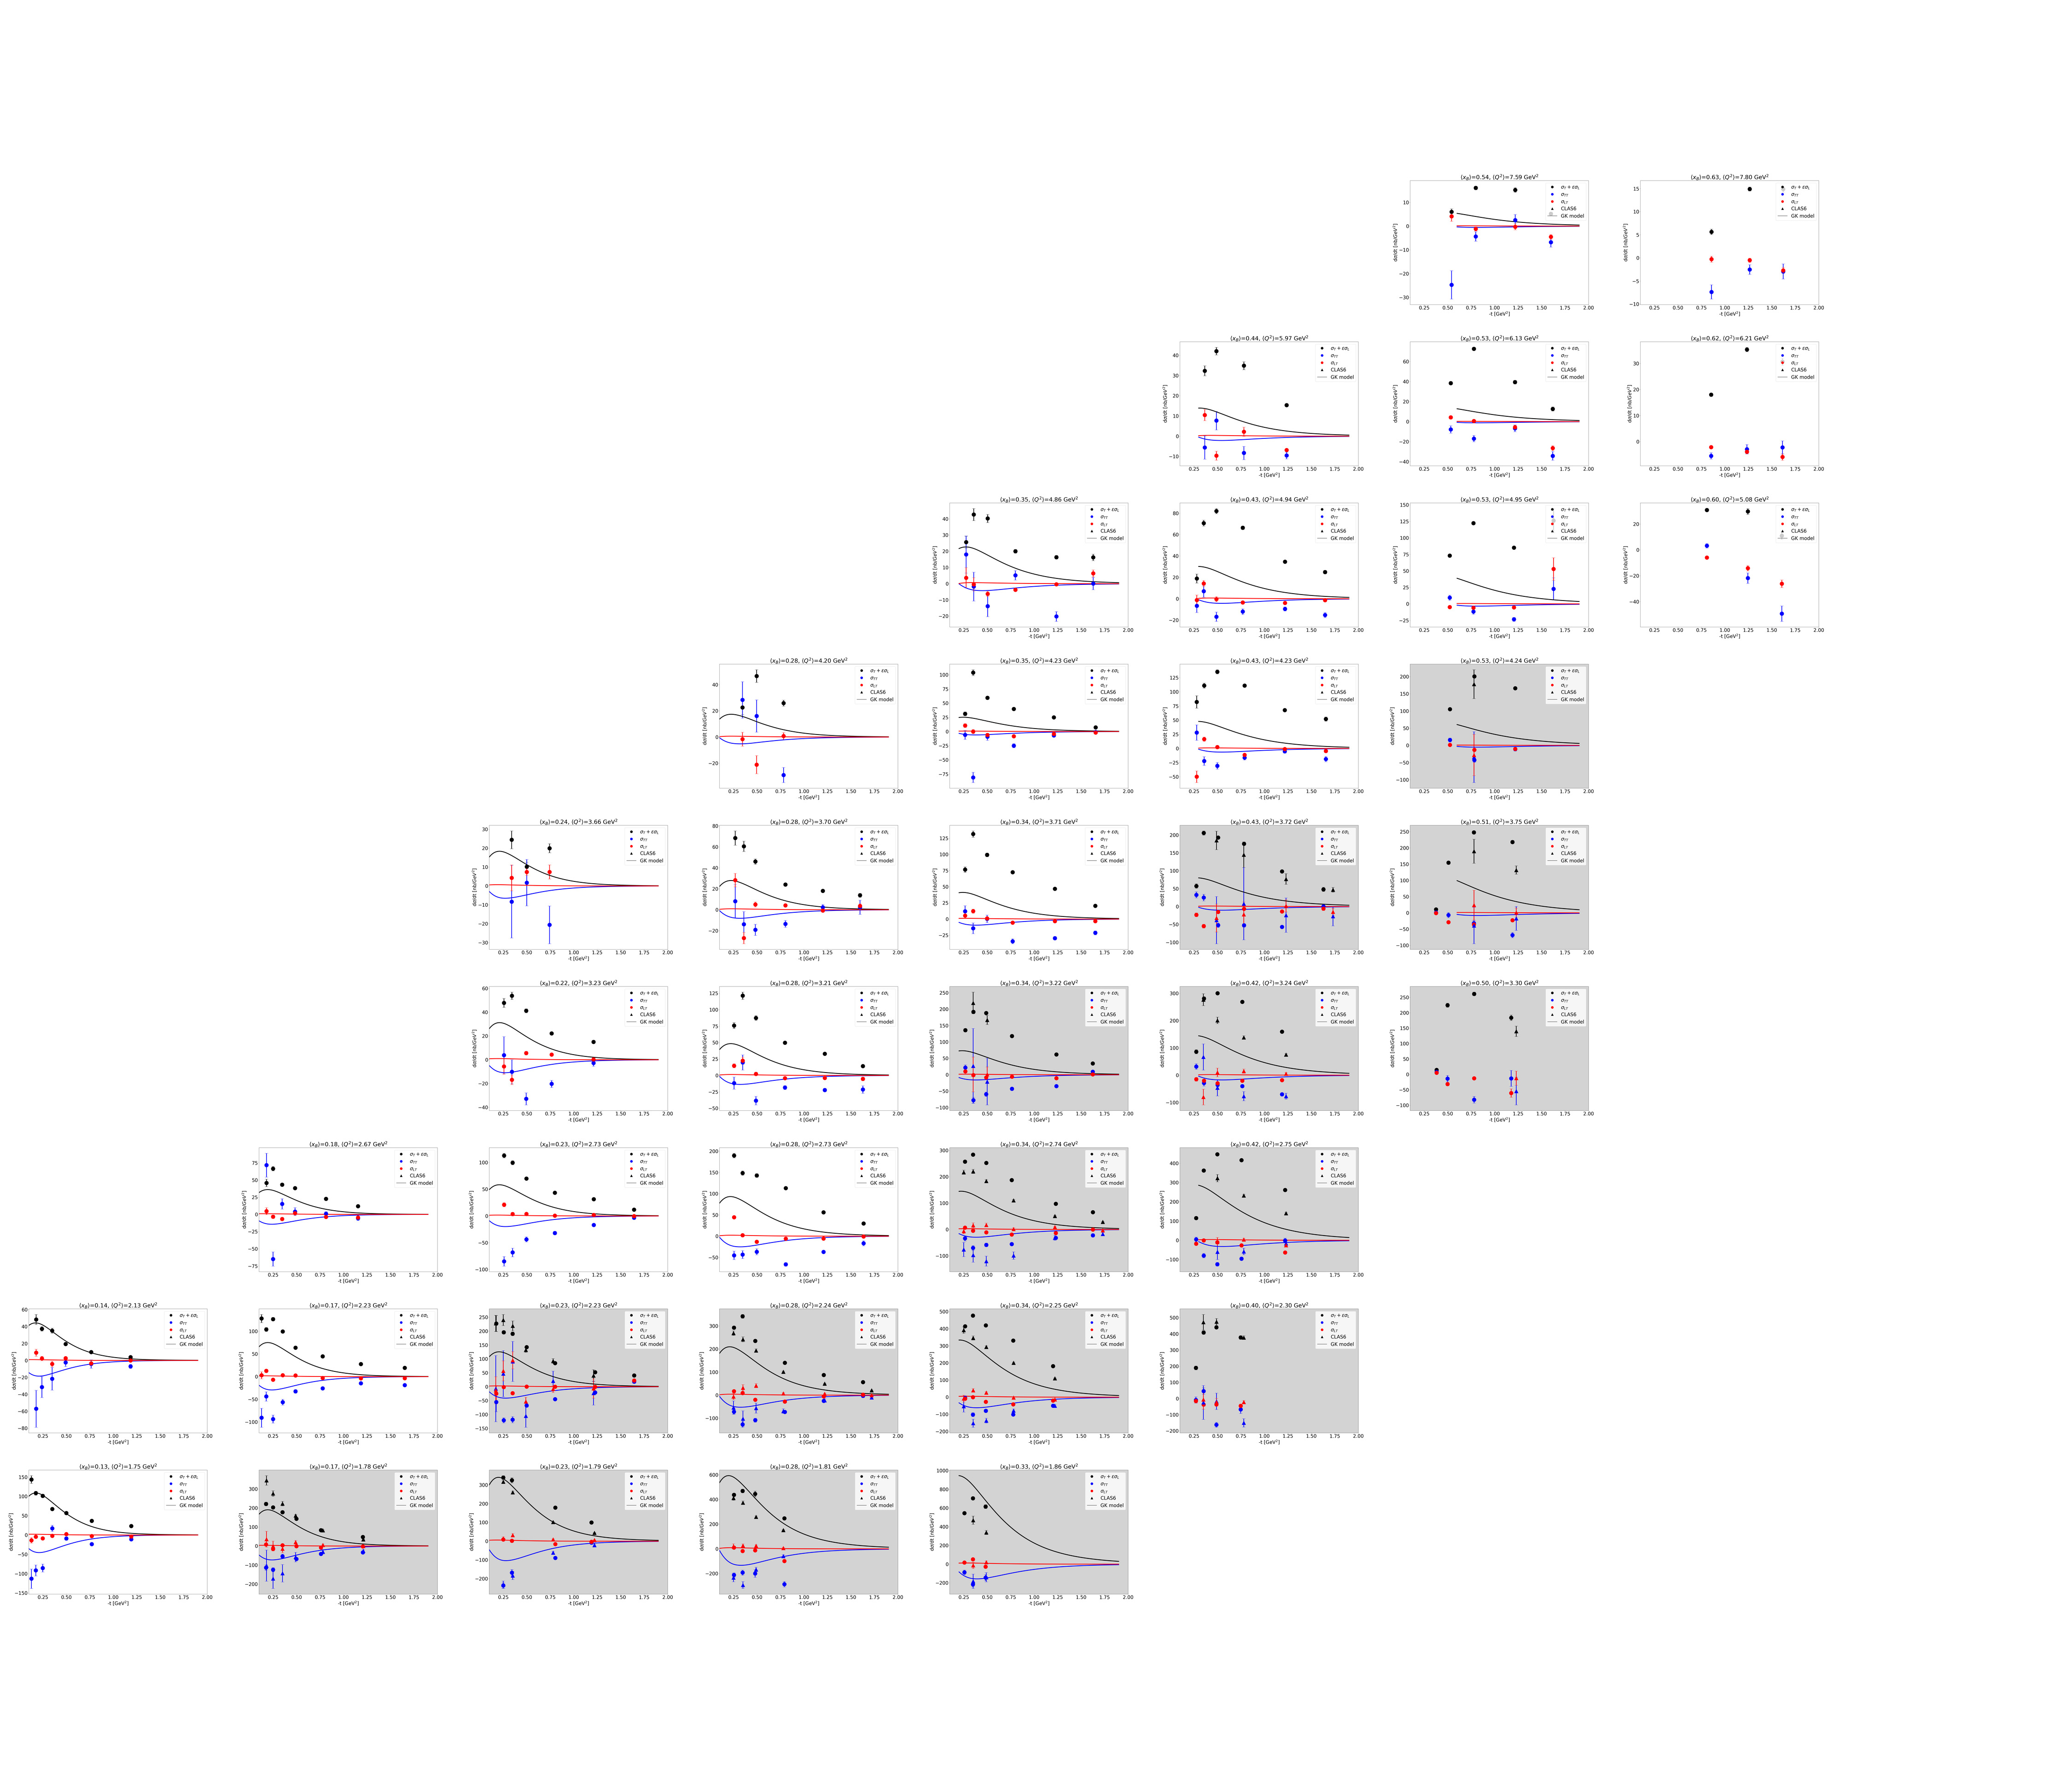
\includegraphics[trim={0 15cm 18cm 13cm},clip,angle=90,origin=c,width=0.85\textwidth]{Chapters/Ch5-Further/GK_model/pics/combined_t_nofold.png}
        \caption[T Dependence of Cross Section]{Structure Function T Dependence. Gray background = kinematic overlap between CLAS12 and CLAS6. Curves are from the GK model. Uncertainties shown are from fitting functions only.}
        \label{fig:t_dependence}
    \end{figure}
    
    
    \iffalse
        Thank you very much for your response. I include two short responses, below, as well as a third response/question that I hope you can read and respond to: 
        
    \begin{itemize}
        \item Thank you for the reference about the Mandelstam function. I was afterwards able to also find reference to it here, where it was named Kallen Function. I haven't heard of either names before. Thanks! \href{https://en.wikipedia.org/wiki/K%C3%A4ll%C3%A9n_function}{Källén Function on Wikipedia}
    
        \item Yes, I am using the code for $\pi^0$, so I do not believe any changes need to be made. I am just working from the single C++ file, since it is easier than getting set up with a full partons framework which looked like it had some overhead to setup and install.
    \end{itemize}



    The Goloskokov-Kroll model has been phenomenologically successful (inlcude links showing this).  The description is based on QCD factorization theorems. In factorizable processes, the amplitudes can be written as a convolution of a hard scattering which is computable in pQCD, and a soft non perturbative part parameterized by GPDs. Chiral-even GPDs are accessible through DVCS where factorization was proven (CITE). Chiral-odd GPDs can be accessed at subleading twist through Deeply Virtual Meson Production if one assumes an effective handbag mechanism, as descried by the GK model. 
    QCD factorization theorem for DVMP process has only been proven for longitudinally polarized photons, and also that the cross section is suppressed by a power of 1/Q for transversley polarized photons. 
    The GK model computes contributions from transversely polarized photons in the handbag mechanism as a twist-3 effect in which teh soft part of the process is parameterized in terms of Chiral Odd GPDs.
    Several GK model parameters implemented in teh PARTONS framework differ from teh parameters used in refrences. The GK model parameters implemented are used in two different publicatoins
    The GK model, under the assumption of flavor-symmetric sea GPDs, only valence quark GPDs Htilda Etilda Ht and Etildat are needed to describe teh process in the kinematical region of large Q2 but small zai and t. GPDs in teh GK model are constructed from double distribtuions as follows, which can be integrated analytically, and the GPDs can be expressed in teh following form:
    \fi

    

    \iffalse
    
    \textbf{Important question:} I now understand that you took the most updated parameters from P Kroll that would best describe the JLab kinematics from the 2020 paper, and that these are different from the parameters available in 2013. My question to you is - are the parameters that are currently implemented in the GK model the best parameters for me to use (for calculating $\pi^0$ cross section at JLab CLAS12 10.6 GeV experiment)? Do you take into account any other experiments (such as work in hall A or C) for finding the parameters? To say it differently, how are optimal parameters chosen for this model?
    
    I would refrain myself speaking on behalf of the authors on that question. They might give you better insights into their model. But I can tell you my viewpoint. I think the GPDs should not be optimized for your data. What I mean is the following: since GPDs are universal functions, ideally there should not be multiple parameters for different experiments (so that we have the flexibility to choose among different parameter sets). Rather, the more data we get, the better parameters need to be determined and those parameters need to be unique for all experiments. In this regard, I would just use the latest parameters that the authors offer (assuming that they did a global analysis to tune those parameters). You could alternatively try to change the parameters to fit them to your data and suggest how your data will impact the extraction of the parameters.
    
    I hope it makes sense, otherwise, we could discuss it further.
    
    Sorry for the late reply. During the last few weeks, I had some other tasks to complete. I'll be happy to share my thoughts with you.
    
    \begin{enumerate}
        \item I think the difference is just the different parameters used in separate works. The parameters of GPDs and their t-slope are not completely the same. At the time I wrote the code, I took the most updated parameters from P. Kroll (or parameters that he thought would best describe the JLab kinematics in Fig. 3 of \href{https://arxiv.org/pdf/2007.15677.pdf}{this paper}). So, I would not expect the same curves just because the GPDs in those works have different parameters.
    
        \item The function $\Lambda$ is called the Mandelstam variable and somehow I could not find the generic expression online. But, I expressed the definition in my thesis (see Eq. 4.50 on page 129); \href{https://www.osti.gov/biblio/1881460}{this link} therein (Chapter 4) you can also see a more detailed implementation of the model. The value of 0.3894 comes from the conversion from $\text{GeV}^{-2}$ to mb.
    
        \item Yes, the final code works for both $\pi^+$ and $\pi^0$ (I am not sure which one you use; if you use the one that you shared above, then it would work only for $\pi^0$. $\pi^+$ implementation can be found in the PARTONS v3. or I have the code for $\pi^+$ similar to the $\pi^0$ that you shared above). Their formulation is quite similar albeit with important differences. First of all, the $\pi^0$ production does not include the so-called pion-pole contribution (see Eq. 4.39 - 4.42 in my thesis). Moreover, their handbag contributions are slightly different. Their differences at the handbag level are discussed in Eq. 4.37 and 4.38 in my thesis.
    \end{enumerate}
    
    Just let me know if you need any further clarification; I'll be happy to address it.    
    
    
    
    
    \begin{figure}[hbt]
    	\centering
    	\includegraphics[page=6,width=0.6\linewidth]{Chapters/Ch5-Further/GK_model/pics/clas6comp.jpg}
    \end{figure}\label{fig:oldres}
    
    To validate the model, we ran the implementation to generate curves and compared to the published CLAS6 result. We observed that the sigma T and sigma L terms were comparable, but not exactly the same, as the 2014 published results, while the sigma TT term was significantly different. It is believed that these differences are due to improvements in the model made in the past 8 years. Figure \ref{fig:oldres2} shows one example bin of this comparison, where the color of the curves is matched to the corresponding color of the structure functions.
    
    \fi
    
    \iffalse
    
    $
    Their formulation is quite similar albeit with important differences. First of all, the pi0 production does not include the so-called pion-pole contribution (see Eq. 4.39 - 4.42 in my thesis). Moreover, their handbag contributions are slightly different. Their differences at the handbag level are discussed in Eq. 4.37 and 4.38 in my thesis. $
    
    The parameters of GPDs and their t-slope are not completely the same. At the time I wrote the code, I took the most updated parameters from P. Kroll (or parameters that he thought would best describe the JLab kinematics in Fig. 3 of \parencite{Diehl2020ExtractionKinematics} ). So, I would not expect the same curves just because the GPDs in those works have different parameters. 
    
    Lambda is defined as: %$https://en.wikipedia.org/wiki/Källén_function$
    
    Description of GK by Kemal Thesis:
    
    The Goloskokov-Kroll model has been phenomenologically successful (inlcude links showing this).  The description is based on QCD factorization theorems. In factorizable processes, the amplitudes can be written as a convolution of a hard scattering which is computable in pQCD, and a soft non perturbative part parameterized by GPDs. Chiral-even GPDs are accessible through DVCS where factorization was proven (CITE). Chiral-odd GPDs can be accessed at subleading twist through Deeply Virtual Meson Production if one assumes an effective handbag mechanism, as descried by the GK model. 
    QCD factorization theorem for DVMP process has only been proven for longitudinally polarized photons, and also that the cross section is suppressed by a power of 1/Q for transversley polarized photons. 
    The GK model computes contributions from transversely polarized photons in the handbag mechanism as a twist-3 effect in which teh soft part of the process is parameterized in terms of Chiral Odd GPDs.
    Several GK model parameters implemented in teh PARTONS framework differ from teh parameters used in refrences. The GK model parameters implemented are used in two different publicatoins
    The GK model, under the assumption of flavor-symmetric sea GPDs, only valence quark GPDs Htilda Etilda Ht and Etildat are needed to describe teh process in the kinematical region of large Q2 but small zai and t. GPDs in teh GK model are constructed from double distribtuions as follows, which can be integrated analytically, and the GPDs can be expressed in teh following form:
    
    
    From Easy as Pi:
    Among the many important consequences is the fact that differently from both inclusive and semi-inclusive processes, GPDs can in principle provide essential information
    for determining the missing component to the nucleon longitudinal spin sum rule, which
    is identified with orbital angular momentum. A complete description of nucleon structure
    %requires, however, also the transversity (chiral odd/quark helicity-flip) GPDs, HT (x, ξ, t),
    %ET (x, ξ, t), HeT (x, ξ, t), and EeT (x, ξ, t) [1]. J
    
    
    \begin{figure}[hbt]
    	\centering
    	\includegraphics[page=6,width=0.6\linewidth]{Chapters/Ch5-Further/GK_model/pics/2022_vs_2014_GK_model.jpg}
    \end{figure}\label{fig:oldres2}
    
    Finally, we compare the preliminary CLAS12 reduced cross section to the predictions from the GK model. Sample plots are shown below. Agreement is close but not exact. The functional form is as expected. It is unclear if the offset between the CLAS12 fit and the GK model is due to a model discrepancy, or an absolute normalization uncertainty in the CLAS12 calculation. More quantitative statments will be made when uncertainties and correction factors in the CLAS12 work are better understood.
    \begin{figure}[hbt]
    	\centering
    	\includegraphics[page=6,width=0.45\linewidth]{Chapters/Ch5-Further/GK_model/pics/reduced_xsec_1.5_2_0.2_0.25_0.2_0.3.png}
    	\includegraphics[page=6,width=0.45\linewidth]{Chapters/Ch5-Further/GK_model/pics/reduced_xsec_1.5_2_0.25_0.3_0.2_0.3.png}
    \end{figure}\label{fig:oldres4}

    \fi
    
    
    \iffalse
    %Notes from PAC UPdate on GL model (NOT GK)
    In general, there are 8 spin-dependent quark-nucleon GPDs, 4 chiral even and 4 chiral odd \parencite{8}. The early efforts to explain $\pi_0$, $\eta$ electroproduction focused on the chiral even $H$, $e Ee$ as a means to parametrize only the longitudinal virtual photon amplitudes \parencite{7}. However, in the approach of Goldstein, Liuti and collaborators \parencite{9} (GL), the quantum numbers and Dirac structure of $\pi_0$ electroproduction restrict the possible contributions to the 4 chiral odd GPDs, one of which, $H_T$, is related to the transversity distribution and the tensor charge. The GL approach leads to sizable transverse photon amplitudes, as indicated in early Hall B data. The reasoning involves the $t$-channel perspective in which the leading contributions to $\pi_0$ will have $J P C 1^{-−}$ and $1+−$, i.e. $C$-parity odd, Parity odd or even. The transverse photon receives contributions from both, while longitudinal photons couple primarily to the axial vector components. To see the implications of these observations for the GPDs entering $\pi_0$ exclusive electroproduction, we use the helicity amplitude formalism. By working out the connection between the $t$-channel and the $s$-channel $J P C$ quantum numbers one can see the relevance of the chiral odd GPDs.
    
    These results have interesting consequences. In a factorized handbag picture, the chiral odd GPDs will couple to the hard part, $\gamma^{*} +$ quark $\rightarrow \pi_0 +$ quark, providing the $\pi_0$ couples through $\gamma^5$, which is naively twist 3, rather than the twist 2 $\gamma^+ \gamma^5$. Nevertheless, the previous arguments support this choice. In \parencite{9} a new model was proposed, using crossing symmetry and duality, which connected the hard subprocess amplitude with the $\gamma^{*}(qq\overline{q}) \rightarrow \pi_0$ vertex. This introduces OAM in the vertex structure. In the transition between the vector mesons $J P C = 1^{−−}$, and the $\pi_0$, $J P C = 0^{−+}$, the quark-antiquark pair carries OAM $L = 0$, both in the initial and final state ($\Delta L = 0$). The transition between the axial-vector mesons $J P C = 1^{+−}$, and the $\pi_0$, is instead characterized by a change of OAM ($\Delta L = 1$). This transition corresponds to larger spatial partonic configurations, and is therefore suppressed of $O(1/Q^2)$. Summarizing, the distinction between the $J P C$ quantum numbers in the $t$-channel allows also for a more flexible model of the $Q^2$ and $x_B$ dependence of deeply virtual exclusive processes. New predictions were more recently obtained (see Fig.4) by extending the physically motivated parametrization for the GPDs of Refs.\parencite{11, 25} to the chiral-odd sector.
    
    This parametrization uses the quark-diquark model, and it has Regge behavior at small $x$. The GPD model parameters are constrained by data on PDFs (at $\zeta = 0$, $t = 0$), $H^q (X, 0, 0) = f^q_1 (X)$, $\tilde{H}^q (X, 0, 0) = g^q_1 (X)$, $H^q_T (X, 0, 0) = h^q_1 (X)$ on nucleon form factors $F_1(t)$, $F_2(t)$, $g_A(t)$, $g_P (t)$, and by recent DVCS measurements \parencite{2} \parencite{3}. Since chiral odd GPDs are much more loosely constrained by experiments – the most “robust” constraint is provided by transversity – $H_T (x, 0, 0) = h_1(x)$ – a very important result of the new GL reggeized diquark approach \parencite{10} is that using helicity amplitudes the chiral odd GPDs are directly related to the chiral even GPDs, thus providing the otherwise missing normalizations for the latter.
    
    As a result, with the GL ansatz all observables can be determined (in parallel with corresponding Regge predictions), extending the initial work \parencite{9} with far more extensive parameterization, and several new predictions \parencite{11, 10}. (Recently a similar emphasis on chiral odd contributions for $\pi$ electroproduction has been proposed \parencite{5}, although the details of that model are quite different.) An example of the GL cross sections at one set of measured kinematics are displayed in Fig. 4.
    \fi



\clearpage
\section{Impact Parameter and t Dependence}
    
    The t dependence of the differential cross section $d\sigma_U/dt$ can also be calculated by integrating the reduced cross sections over $\phi$ as \eqref{eq:tdep}
    
     \begin{equation}\label{eq:tdep}
        \frac{d\sigma_U}{dt} = \int \frac{d^2\sigma}{dtd\phi} d\phi.
    \end{equation}
    
    In order to account for regions where the CLAS12 detector system has zero acceptance, it is necessary to include a correction factor $\eta'$, defined as \eqref{eq:eta}
    
     \begin{equation}\label{eq:eta}
        \eta' = \frac{\int_{\Omega*} \frac{d^2\sigma}{dtd\phi} }{\int_{\Omega} \frac{d^2\sigma}{dtd\phi}}.
    \end{equation}

    $\eta'$ is calculated through simulation; in order to not introduce too much model bias we restrict analysis to t bins where the coverage in $\phi$ was greater than 50\%. The cross sections are then fit with the exponential form $Ae^{-bt}$, where b is the Fourier transform of the impact parameter in the handbag model. The results are shown in \figref{fig:bslopes}. The $Q^2$ and $x_B$ dependencies are as expected from theory and this work shows good agreement with the results of previous CLAS6 work \parencite{Bedlinskiy2014ExclusiveCLAS}. %of th eWe observe a good agreement in the b slope parameter, which describes the width of the transverse momentum distribution of the proton, between CLAS12 and the published CLAS6 data.

    \begin{figure}[hbt]
    	\centering
    	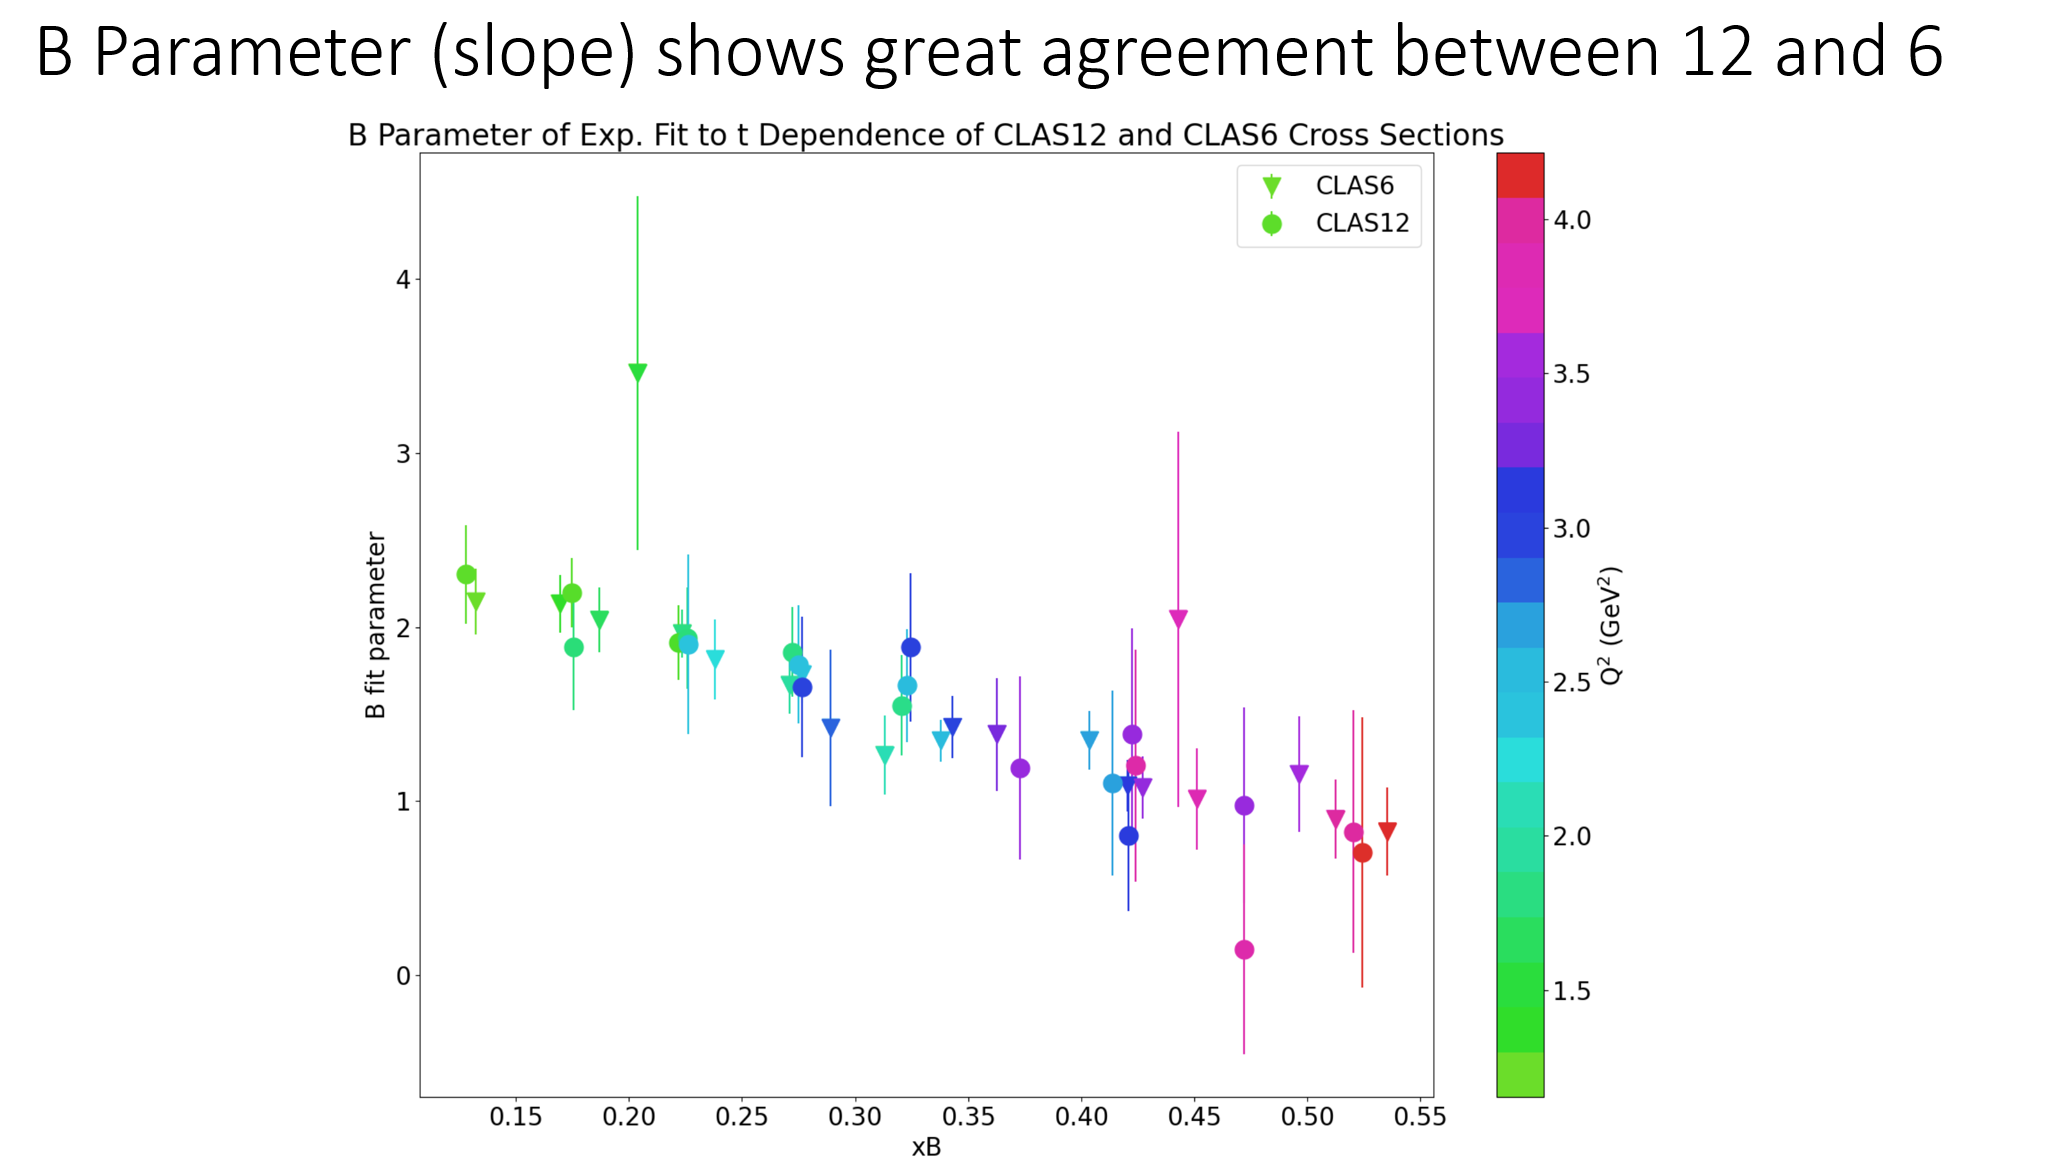
\includegraphics[trim={0 0 0 2.1cm},clip,width=0.8\linewidth]{Chapters/Ch5-Further/t_dependence/pics/bslopes.png}
    
    	\caption[Impact Parameter B]{CLAS12 (this work) and CLAS6 \parencite{Bedlinskiy2014ExclusiveCLAS} t dependence of cross sections. The fits are exponential functions $Ae^{-bt}$, where the slope parameter b are in close agreement for the bins considered.}
    	\label{fig:bslopes}
    \end{figure}
    

    


%\section{Rosenbluth Separation Between Beam Energies}
%    \input{Chapters/Ch5-Further/Rosenbluth_Separation/Rosenbluth_Separation}

\clearpage
\section{Conclusion}

    We have presented the Deeply Virtual $\pi^0$ Production over a wide kinematic range. The DV$\pi^0$P cross section is in reasonable agreement with previous measurements in regions where there is kinematic overlap, as well as with the leading theory parametrization at low $Q^2$. Deviations from the model as $Q^2$ increases is a known effect. The cross sections $\phi$ dependence is as expected from the handbag model. From inspecting \figref{fig:t_dependence} we observe that $\frac{\sigma_{LT}}{dt}$ is small in comparison with $\frac{\sigma_{TT}}{dt}$ and  $\frac{d\sigma_T}{dt} + \epsilon \frac{d\sigma_L}{dt}$, which is consistent with previous results. % and indicates 
    This result leads to the direct availability of performing a Rosenbluth separation to disentangle the $\sigma_L$ and $\sigma_T$ terms, as was recently  performed on the CLAS6 dataset \parencite{Korover2021RosenbluthProton}
    %\parencite{Korover2021RosenbluthProton}. 
    Relatedly, work will continue collaboration-wide to validate detector efficiencies and absolute normalization, which will reduce the systematic uncertainties of this measurement. Efforts are also continuing on the unfolding methods, in particular there is collaboration interest in pursuing an unbinned unfolded cross section \parencite{Andreassen2020OmniFold:Observables} which would further reduce uncertainties and facilitate future analysis efforts. 
        
    %The result is consistent with the expected result from quark transversity GPDs and QCD factorization theorems. 

     %sigma L vs sigma T
     
    This measurement represents the first DV$\pi^0$P electroproduction off a proton cross section measurement at the CLAS12 experiment, with many more expected in the coming years at varying beam energies and set ups. More broadly, nucleon imaging work will continue for years to come at JLab and facilities around the world \figref{fig:physics_future_ranges}, notably at the upcoming Electron-Ion Collider (EIC) which reaches deep into the low-x territory while also overlapping with the kinematics discussed in this work. 

    \begin{figure}
        \centering
        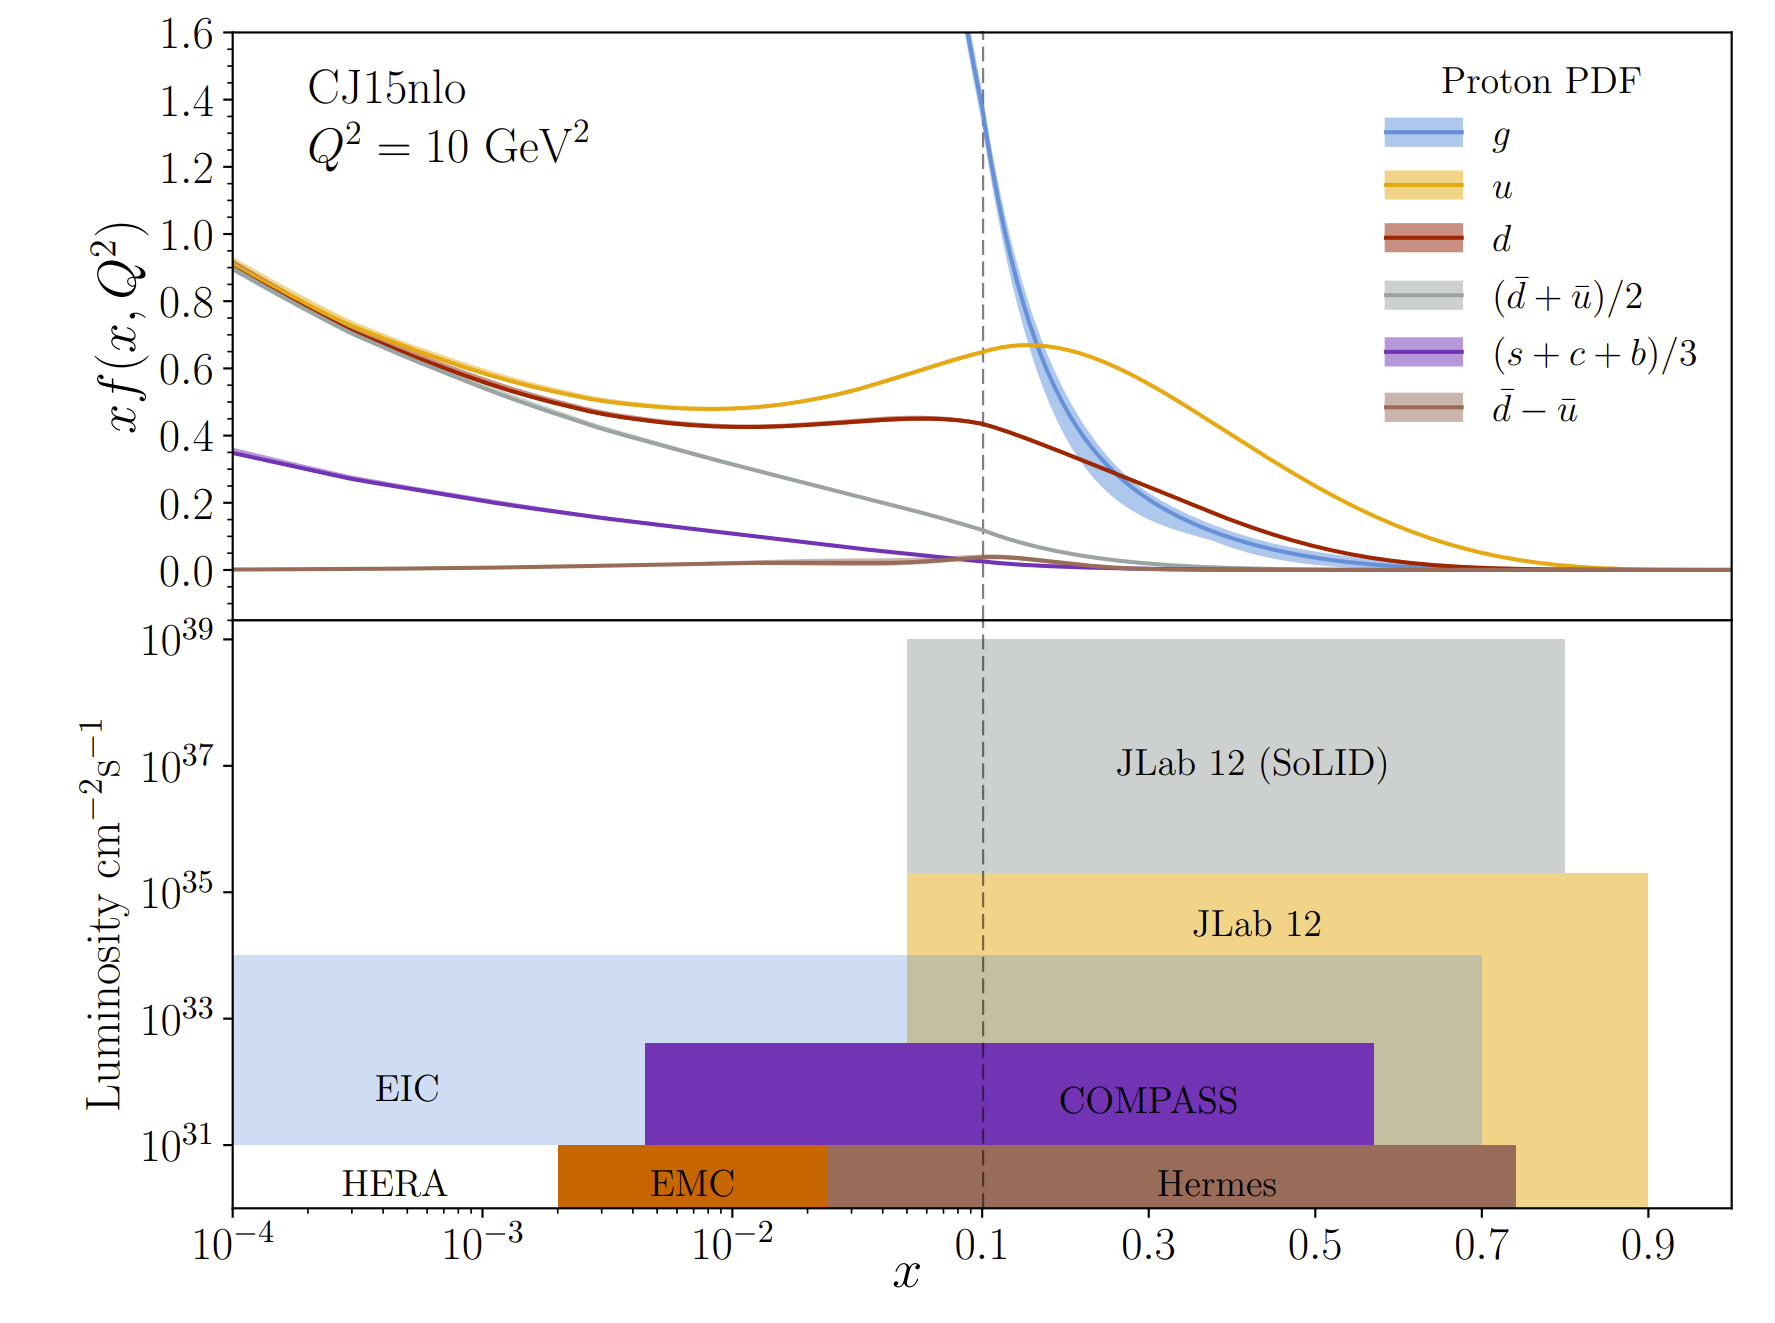
\includegraphics[width=0.9\textwidth]{Chapters/Ch5-Further/X_conclusion/pics/future.png}
        \caption[Kinematic Overlap of Future Experiments]{Kinematic regions of Deep Inelastic Scattering and the comparative reach of EIC and CEBAF, from \parencite{Arrington2022PhysicsOpportunities}. }
        \label{fig:physics_future_ranges}
    \end{figure}












\iffalse

    \
    \begin{figure}[hbt]
    	\centering
    	\includegraphics[page=125,width=0.45\linewidth]{Chapters/Ch5-Further/t_dependence/pics/fig_1.0_0.15.png}
    	\includegraphics[page=130,width=0.45\linewidth]{Chapters/Ch5-Further/t_dependence/pics/fig_1.5_0.15.png}
    
    	\caption[t dependence]{CLAS12 and CLAS6 t dependence of cross sections. The fits are exponential functions $Ae^{-bt}$, where the slope parameter b are in close agreement for the bins considered. The overall normalization A is not yet determined for the CLAS12 dataset, so a small overall offset from the CLAS6 data is expected. Errors are only statistical.}
    	\label{fig:tdep}
    \end{figure}
    \

    
    Omnifold, Miguel Arretahg
    indicate adjustments to GK model 
     "Continuous
    studies based on the current and future measurements will make possible new insights
    into the QCD structure of hadronic matter."
    
    Rosenbluth separation - not very large
    
    
    Comment on factorization theorem and sigma L vs sigma T
    
    OMNIFold method
    
    Pass1 data suffer from CD mis-alignment and other issues solved in the new cooking
    
    
    Despite that, you might be able to perform the LT separation and get Q\^2 and t dependences of dσU as Hall A guys did. And, the most important thing is to argue that you found that result is consistent or not with the expected result from the quark transversity GPDs!!!!!!!!!. The normalization issue is only adding the multiplicative uncertainties on C at Table II of the Hall A PRL paper for example. And, Richard will be doing his best to hide euphoria, and you hand shake with him. Done.
    
    
        Yes, that is the reference. You saw that I also posted a reference to the Hera analysis. I don’t think many others have used omnifold yet, since it is quite computationally intensive etc.
    My understanding is that Ben Nachman developed this and there has been follow up work by his group (if you just put his name into inspire you’ll see). E.g. I saw presentations on how to present the data. Here is a talk by Ben at a Jet workshop in 2021: \href{https://indico.bnl.gov/event/10555/contributions/54721/attachments/37368/61570/H1Measurement_EICWorkshopSeptember2021.pdf}{this paper}
     Miguel Arratia, who is also in CLAS collaborated on the H1 results. You could ask him for practical advice,
    


    \fi









